%% Author: Leighton Pritchard
%% Copyright: James Hutton Institute
%% 2016-03-21: Slides for Software Sustainability institute RDVW, 28th July 2016
%% This presentation was an invited lecture for a research visualisation workshop,
%% to last 30min before a 2hr 'hands-on' session

%% UNCOMMENT FOR SLIDES
\documentclass[table]{beamer}
\mode<presentation>

%% UNCOMMENT FOR HANDOUTS
%\input{sections/preamble_handouts}
%% GENERIC STYLE SETTINGS BELOW
\usetheme{default}
\usepackage{listings}
\usepackage{multirow}
\usepackage{xcolor}
\usepackage{hyperref}
\usepackage{eurosym}
\usepackage[export]{adjustbox}
%\usepackage[multiple]{footmisc}

%% BACKGROUND TEMPLATE
\usebackgroundtemplate{

\includegraphics[width=\paperwidth,height=\paperheight]{images/hutton_background}
}

%% PRESENTATION CONFIGURATION PARAMETERS %%%%%%%%%%%%%%%%%%%
%\titlebackgroundfile{images/hutton_title}
%\framebackgroundfile{images/hutton_background}
\definecolor{hutton_green}{HTML}{78A22F}
\definecolor{hutton_purple}{HTML}{872175}
\definecolor{hutton_blue}{HTML}{569BBE}
\definecolor{olive}{rgb}{0.3, 0.4, .1}
\definecolor{fore}{RGB}{249,242,215}
\definecolor{back}{RGB}{51,51,51}
\definecolor{title}{RGB}{255,0,90}
\definecolor{dgreen}{rgb}{0.,0.6,0.}
\definecolor{gold}{rgb}{1.,0.84,0.}
\definecolor{JungleGreen}{cmyk}{0.99,0,0.52,0}
\definecolor{BlueGreen}{cmyk}{0.85,0,0.33,0}
\definecolor{RawSienna}{cmyk}{0,0.72,1,0.45}
\definecolor{Magenta}{cmyk}{0,1,0,0}
\usefonttheme{structurebold}
\setbeamercolor{alerted text}{fg=orange}
\setbeamercolor{background canvas}{bg=white}
\setbeamercolor{block title}{bg=hutton_purple}
\setbeamercolor{frametitle}{fg=hutton_purple}
\setbeamercolor{title}{fg=black}
\setbeamercolor{titlelike}{fg=hutton_green}
\setbeamercolor{author}{fg=hutton_purple}
\setbeamercolor{author in head/foot}{fg=white}
\setbeamercolor{title in head/foot}{fg=white}
\setbeamercolor{section in head/foot}{fg=hutton_purple}
\setbeamercolor{normal text}{fg=black}
\setbeamercolor{frametitle}{fg=hutton_purple}
\setbeamerfont{author}{size=\footnotesize}
\setbeamerfont{institute}{size=\tiny}
\setbeamerfont{date}{size=\footnotesize}
\setbeamercolor{section in toc shaded}{fg=hutton_purple}
\setbeamercolor{section in toc}{fg=hutton_purple}
\setbeamercolor{subsection in toc shaded}{fg=hutton_purple}
\setbeamercolor{subsection in toc}{fg=hutton_purple}
\setbeamertemplate{itemize item}[circle]
\setbeamertemplate{itemize subitem}[circle]
\setbeamertemplate{itemize subsubitem}[circle]
\setbeamertemplate{itemize subsubsubitem}[circle]
\setbeamercolor{itemize item}{fg=hutton_purple}
\setbeamercolor{itemize subitem}{fg=hutton_purple}
\setbeamercolor{itemize subsubitem}{fg=hutton_purple}
\setbeamercolor{itemize subsubsubitem}{fg=hutton_purple}
\setbeamercolor{enumerate item}{fg=hutton_purple}
\setbeamercolor{enumerate subitem}{fg=hutton_purple}
\setbeamercolor{enumerate subsubitem}{fg=hutton_purple}
\setbeamercolor{enumerate subsubsubitem}{fg=hutton_purple}

% ALERTS AND BLOCKS
\setbeamercolor{alerted text}{fg=hutton_green}
\setbeamerfont{alerted text}{series=\bfseries}
\setbeamercolor{block title}{use=structure,fg=white,bg=structure.fg!75!black}
\setbeamercolor{block title alerted}{use=alerted text,fg=white,bg=alerted text.fg!75!black}
\setbeamercolor{block title example}{use=example text,fg=white,bg=example text.fg!75!black}
\setbeamercolor{block body}{parent=normal text,use=block title,bg=block title.bg!10!bg}
\setbeamercolor{block body alerted}{parent=normal text,use=block title alerted,bg=block title alerted.bg!10!bg}
\setbeamercolor{block body example}{parent=normal text,use=block title example,bg=block title example.bg!10!bg}

% This command makes sure that acrobat reader doesn't change the colours of the slide
% when there are figures with transparencies.
\pdfpageattr {/Group << /S /Transparency /I true /CS /DeviceRGB>>}

%Disables discrete bottom navigation bar
\beamertemplatenavigationsymbolsempty

% Modify the slide titles to avoid the corner images,
\setbeamertemplate{frametitle}
{
\vspace{0.05\textheight}
\noindent\quad\begin{minipage}[t][0.12\textheight][t]{0.85\textwidth}
\insertframetitle\par
\end{minipage}
}

% Modify title page to avoid the big logo on right
\setbeamertemplate{title page}{
    \begin{picture}(0,0)
            %This ends up on top of the default background image, rather than replacing it:
            \put(-30,-165){%
                
\includegraphics[width=\paperwidth,height=\paperheight]{images/hutton_title}
            }
            \put(0,-75){%
                \begin{minipage}[b][0.4\textheight][t]{0.75\textwidth}
                    \usebeamerfont{title}\usebeamercolor[fg]{title}{\inserttitle\par}
                    \usebeamerfont{subtitle}\usebeamercolor[fg]{subtitle}{\insertsubtitle\par}
                \end{minipage}
            }
            \put(0,-125){%
                \begin{minipage}[b][0.1\textheight][t]{\textwidth}
                    \usebeamerfont{author}\usebeamercolor[fg]{author}{\insertauthor\par}
                    \usebeamerfont{institute}\usebeamercolor[fg]{institute}{\insertinstitute\par}
                \end{minipage}
            }
    \end{picture}
}

% Make \verbatim environment tiny font
\makeatletter
\def\verbatim{\tiny\@verbatim \frenchspacing\@vobeyspaces \@xverbatim}
\makeatother

% Inner Theme for Blocks
\useinnertheme{rectangles}

%%%%%%%%%%%%%%%%%%%%%%%%%%%%%%%%%%%%%%%%%%%%%%%%%%%%%%%%%%%%%%%%%%%%%%%%%%%%%%%%

% LISTINGS SETTING
% Settings for code listings in lstlistings

\definecolor{hutton_lightgreen}{HTML}{C8F27F}

\lstset{ %
  backgroundcolor=\color{hutton_lightgreen},   % choose the background color; you must add \usepackage{color} or \usepackage{xcolor}
  basicstyle=\tiny\ttfamily,        % the size of the fonts that are used for the code
  breakatwhitespace=false,         % sets if automatic breaks should only happen at whitespace
  breaklines=true,                 % sets automatic line breaking
  captionpos=b,                    % sets the caption-position to bottom
  commentstyle=\color{red},    % comment style
  deletekeywords={...},            % if you want to delete keywords from the given language
  escapeinside={\%*}{*)},          % if you want to add LaTeX within your code
  extendedchars=true,              % lets you use non-ASCII characters; for 8-bits encodings only, does not work with UTF-8
  frame=single,                    % adds a frame around the code
  keepspaces=true,                 % keeps spaces in text, useful for keeping indentation of code (possibly needs columns=flexible)
  keywordstyle=\color{blue},       % keyword style
%  language=Octave,                 % the language of the code
  morekeywords={*,...},            % if you want to add more keywords to the set
  numbers=left,                    % where to put the line-numbers; possible values are (none, left, right)
  numbersep=5pt,                   % how far the line-numbers are from the code
  numberstyle=\tiny\color{gray}, % the style that is used for the line-numbers
  rulecolor=\color{black},         % if not set, the frame-color may be changed on line-breaks within not-black text (e.g. comments (green here))
  showspaces=false,                % show spaces everywhere adding particular underscores; it overrides 'showstringspaces'
  showstringspaces=false,          % underline spaces within strings only
  showtabs=false,                  % show tabs within strings adding particular underscores
  stepnumber=1,                    % the step between two line-numbers. If it's 1, each line will be numbered
  stringstyle=\color{violet},     % string literal style
  tabsize=4,                       % sets default tabsize to 2 spaces
  title=\lstname                   % show the filename of files included with \lstinputlisting; also try caption instead of title
}


%%%
% TITLE PREAMBLE
\title[RDVW: Python] % (optional, only for long titles)
{Hands-on session: Python}
\subtitle{Research Data Visualisation Workshop}
\author[Pritchard] % (optional, for multiple authors)
{Leighton~Pritchard$^{1,2,3}$}
\institute[The James Hutton Institute] % (optional)
{
  $^{1}$Information and Computational Sciences,\\
  $^{2}$Centre for Human and Animal Pathogens in the Environment,\\
  $^{3}$Dundee Effector Consortium,\\
  The James Hutton Institute, Invergowrie, Dundee, Scotland, DD2 5DA
}
\date[27th June 2016] % (optional)
{27th June 2016}
\subject{Data Science, Data Analysis, Data Visualisation, Research Data Visualisation, Python, Programming}

%%%
% TOC
% Show table of contents, with current section highlighted,
% at the start of each section

%\AtBeginSection[]
%{
%  \begin{frame}
%    \frametitle{Table of Contents}
%    \tableofcontents[currentsection] %,hideallsubsections]
%  \end{frame}
%}

% TOC AT SECTIONS
%\AtBeginSection[]
%{
%  \begin{frame}
%    \frametitle{Table of Contents}
%    \tableofcontents[currentsection,currentsubsection] %,hideallsubsections]
%  \end{frame}
%}

% TOC AT SUBSECTIONS
\AtBeginSubsection[]
{
  \begin{frame}
    \frametitle{Table of Contents}
    \tableofcontents[currentsection,currentsubsection] %,hideallsubsections]
  \end{frame}
}

%%%
% START DOCUMENT
\begin{document}

\frame[plain]{\titlepage}

%% use.tex
%% Author: Leighton Pritchard
%% Copyright: James Hutton Institute
%% These slides describe the acceptable use policy for these slides and
%% materials

%
\begin{frame}
  \frametitle{Acceptable Use Policy}
  Recording of this talk, taking photos, discussing the content using \\
  email, Twitter, blogs, etc. is permitted (and encouraged), \\
  providing distraction to others is minimised. \\[0.5cm]
  \textbf{These slides will be made available at \href{http://www.slideshare.net/leightonp}{http://www.slideshare.net/leightonp}}
\end{frame}

%%%
% SECTION: INTRODUCTION
\section{Introduction}
\subsection{Why listen to me?}
%% about_me.tex
%% Author: Leighton Pritchard
%% Copyright: James Hutton Institute
%% Why should anyone listen to me, regarding visualisation

% POTTED CV
\begin{frame}
  \frametitle{What I do}
      \begin{itemize}  
        \item \textcolor{hutton_green}{Computational biologist (1996-present)}
        \begin{itemize}
          \item Protein sequence-structure-function (1996-1999)
          \item Yeast metabolism (1999-2003)
          \item Plant pathology (2003-present)
        \end{itemize}
        \item \textcolor{hutton_blue}{Large datasets}
        \begin{itemize}
          \item metabolomics
          \item genomics
          \item geographical
        \end{itemize}
        \item \textcolor{hutton_purple}{Visualisation as communication to (wet) biologists}
        \begin{itemize}
          \item protein structures
          \item metabolic flux
          \item comparative genomics/evolution
        \end{itemize}
      \end{itemize}  
\end{frame}

% GENOMEDIAGRAM
\begin{frame}
  \frametitle{GenomeDiagram 
    \footnote{\tiny{\href{http://dx.doi.org/10.1093/bioinformatics/btk021}{Pritchard \textit{et al.} (2006) \textit{Bioinformatics} doi:10.1093/bioinformatics/btk021}}}
    \footnote{\tiny{Toth \textit{et al}. (2006) \textit{Ann. Rev. Phytopath.} \href{http://dx.doi.org/10.1146/annurev.phyto.44.070505.143444}{doi:10.1146/annurev.phyto.44.070505.143444}}}
    
\includegraphics[width=0.18\textwidth]{images/biopython}
  }
  \begin{center}
      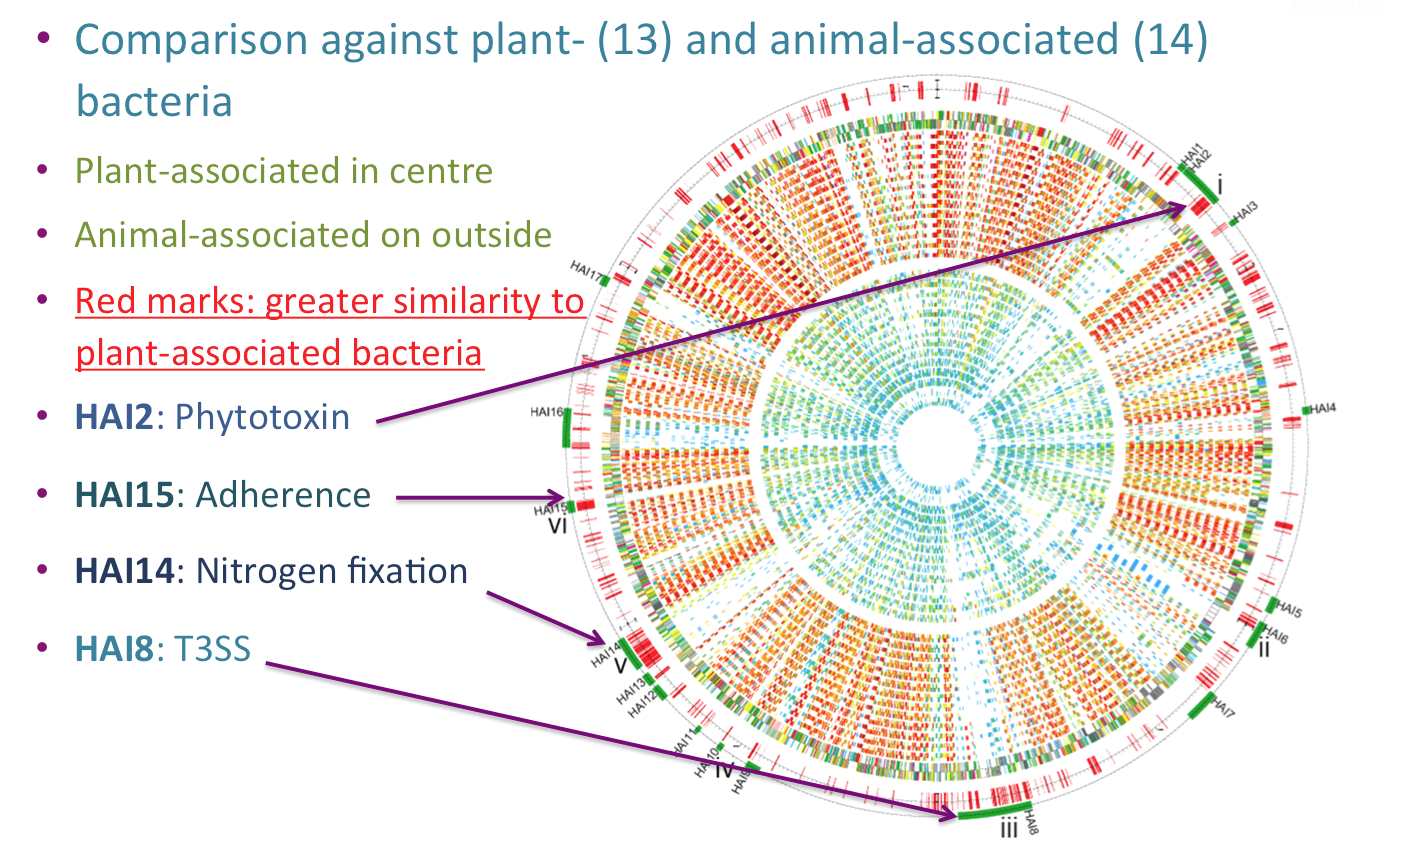
\includegraphics[width=1\textwidth]{images/pba_lgt} 
  \end{center}
\end{frame}

% CORONATINE
\begin{frame}
  \frametitle{Functional adaptation in \textit{Pba}\footnote{\tiny{Toth \textit{et al}. (2006) \textit{Ann. Rev. Phytopath.} \href{http://dx.doi.org/10.1146/annurev.phyto.44.070505.143444}{doi:10.1146/annurev.phyto.44.070505.143444}}}}
  \begin{center}
      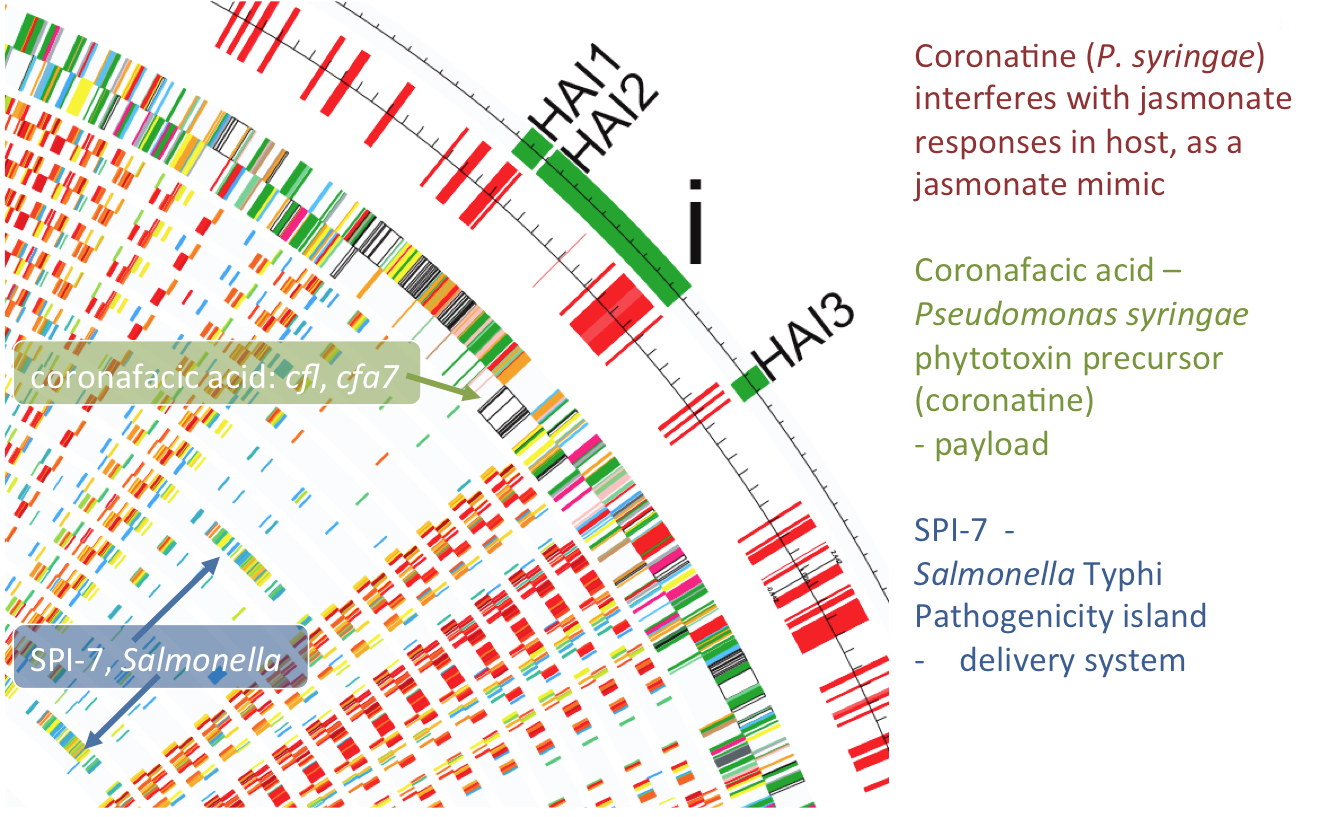
\includegraphics[width=1\textwidth]{images/pba_coronatine} 
  \end{center}
\end{frame}

%% GENOMEDIAGRAM/BIOPYTHON
\begin{frame}
  \frametitle{GenomeDiagram/SciArt
  \footnote{\tiny{\href{http://dx.doi.org/10.1093/bioinformatics/btk021}{Pritchard \textit{et al.} (2006) \textit{Bioinformatics} doi:10.1093/bioinformatics/btk021}}}
  \footnote{\tiny{Shemilt (2009) in``Digital Visual Culture: Theory and Practice'' ISBN 978-1-84150-248-9}}
  \footnote{\tiny{Shemilt (2010) in ``Art Practice in a Digital Culture'', ISBN 978-0-7546-7623-2}}
  }
  \begin{columns}[T]
    \begin{column}{3.5cm}  
%      \includegraphics[height=0.3\textheight]{images/gd_large} \\
      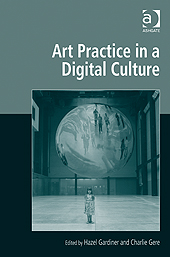
\includegraphics[height=0.4\textheight,center]{images/art_practice}      
        \begin{tiny}    
          \begin{alertblock}{Influence}
            Free open-source comparative genomics visualisation library
          \end{alertblock}                
        \end{tiny}          
        
\includegraphics[width=1\textwidth]{images/biopython}          
    \end{column}    
    \begin{column}{3.5cm}  
      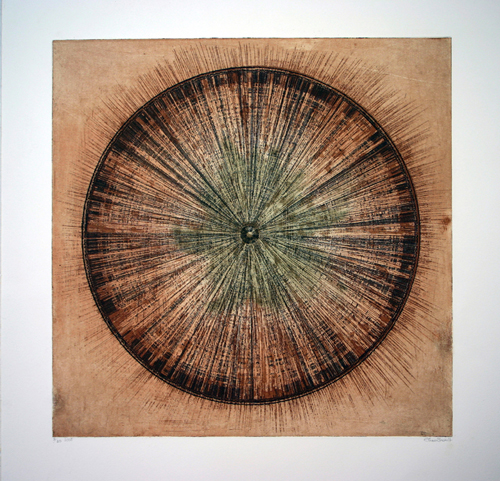
\includegraphics[height=0.4\textheight]{images/shemilt-fig3} \\
        \begin{tiny}        
          \begin{alertblock}{Impact}
            Artwork (prints, audio-visual installation) exhibited in UK and internationally
          \end{alertblock}                
        \end{tiny}                        
    \end{column}
    \begin{column}{3.5cm}  
      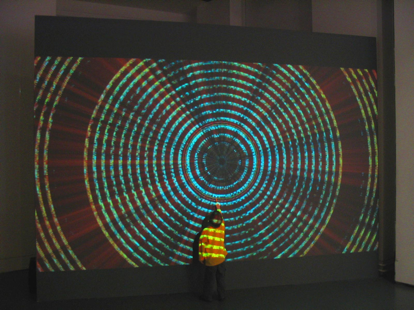
\includegraphics[width=1\textwidth]{images/sciart2} \\
      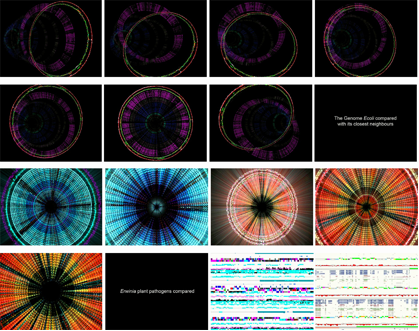
\includegraphics[width=1\textwidth]{images/sciart3}
    \end{column}  
  \end{columns}
\end{frame}

% KGML/KEGG 
\begin{frame}
  \frametitle{Comparative metabolism
    \footnote{\tiny{\href{https://github.com/widdowquinn/notebooks/blob/master/Biopython_KGML_intro.ipynb}{Biopython KGML/KEGG visualisation module}}}
    \footnote{\tiny{\href{https://github.com/widdowquinn/Notebooks-Bioinformatics}{https://github.com/widdowquinn/Notebooks-Bioinformatics}}}
    
\includegraphics[width=0.18\textwidth]{images/biopython}
  }
  \textcolor{hutton_green}{Metabolic potential is a clue to community function \& host range}
  \begin{center}
    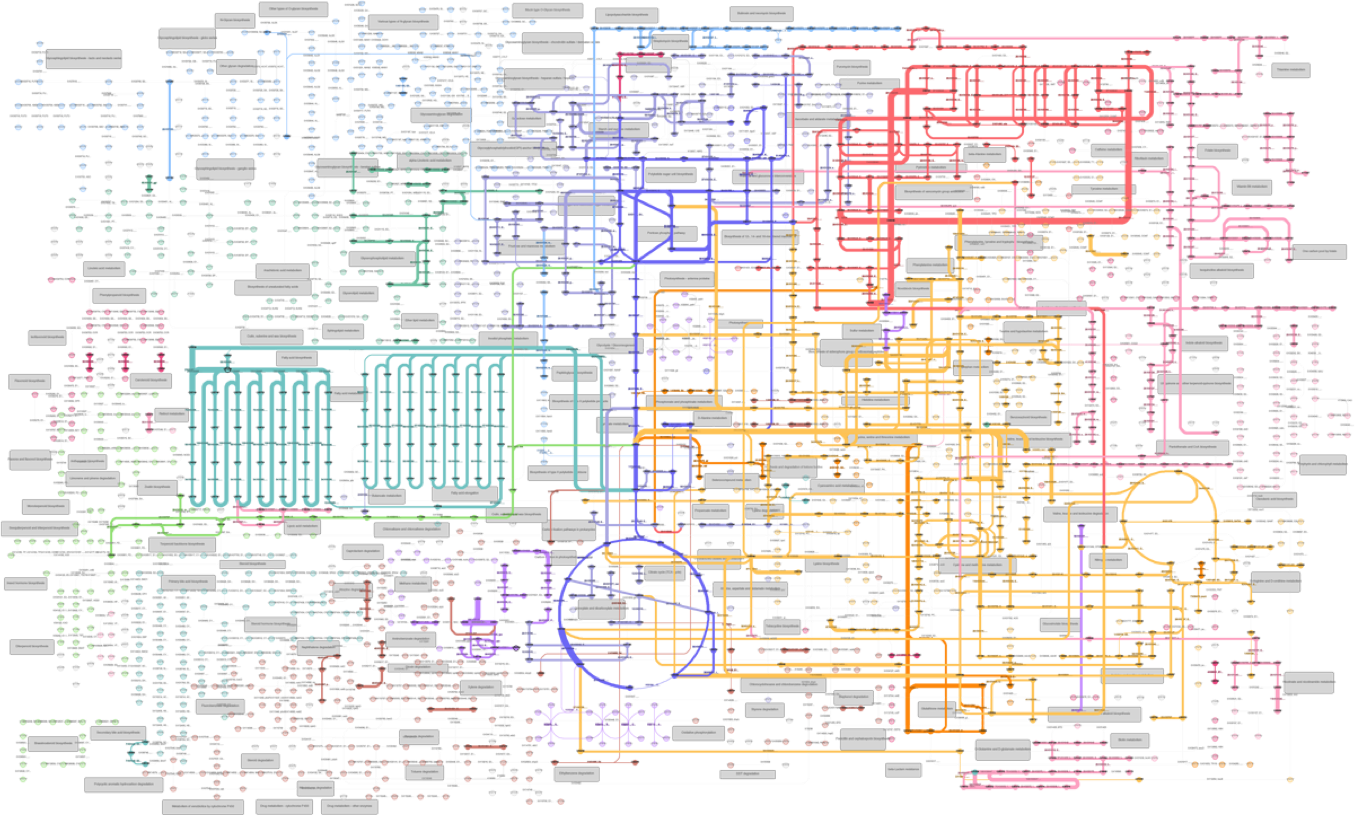
\includegraphics[width=0.9\textwidth]{images/dickeya_pathways}
  \end{center}
\end{frame}

% PYANI
\begin{frame}
  \frametitle{PyANI: prokaryote classification
  \footnote{\tiny{\href{http://widdowquinn.github.io/pyani/}{http://widdowquinn.github.io/pyani/}}}
  \footnote{\tiny{\href{http://dx.doi.org/10.1039/C5AY02550H
}{Pritchard \textit{et al.} (2016) \textit{Anal. Methods} doi:10.1039/C5AY02550H
}}}  
  }
  \begin{center}
    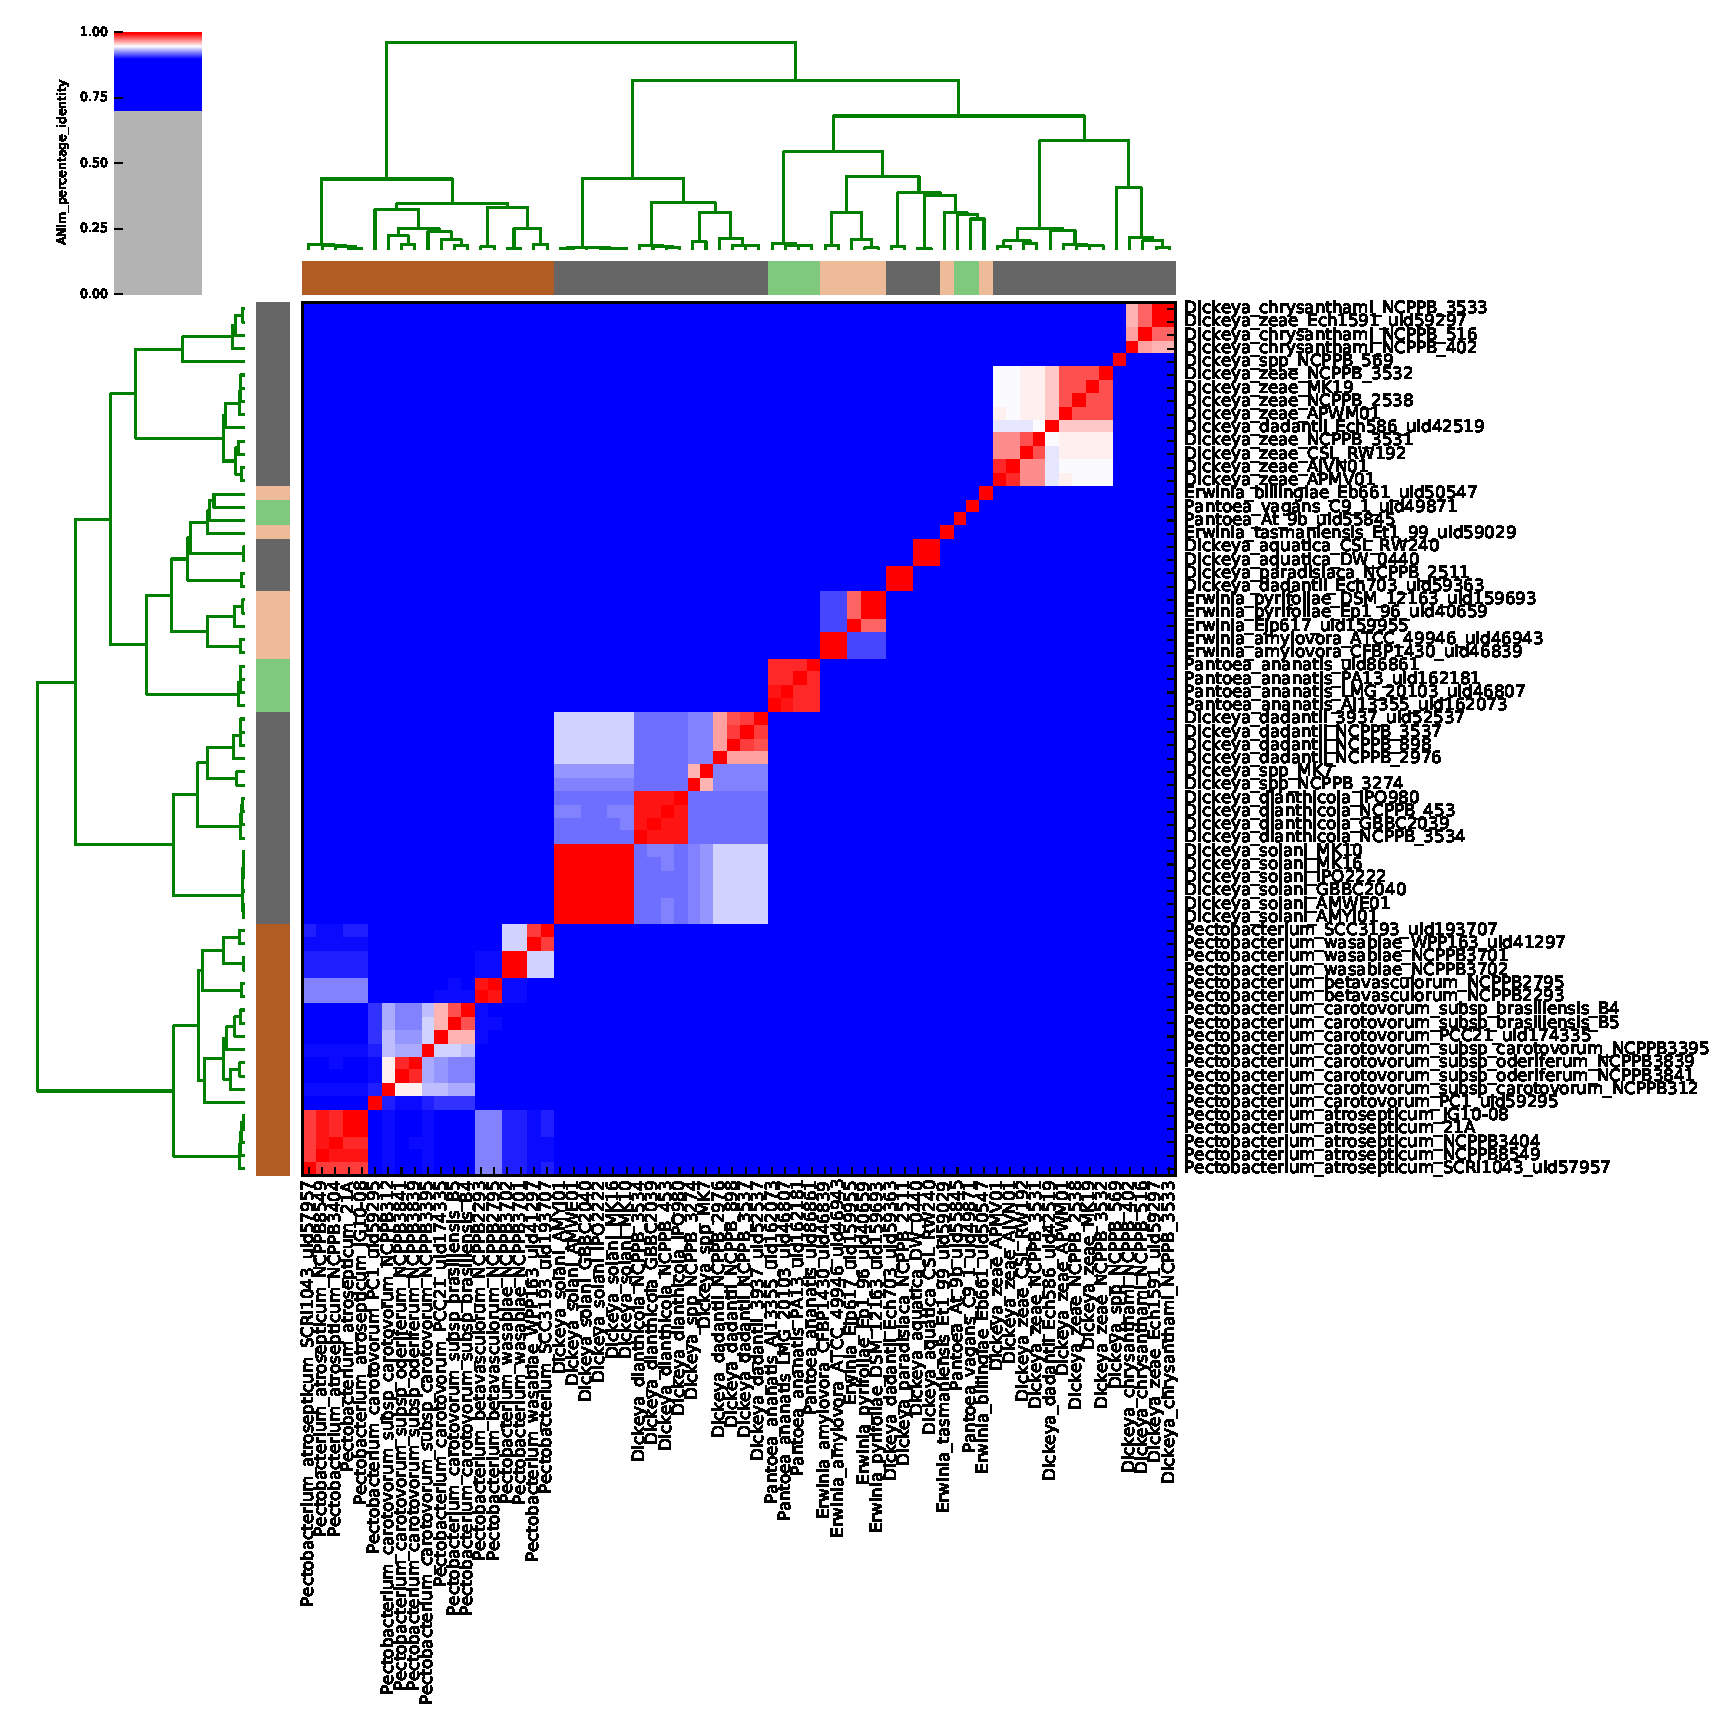
\includegraphics[height=0.75\textheight]{images/figure_anim_pid_SRE}
  \end{center}
\end{frame}
\subsection{What is visualisation?}
%% what_is_datavis.tex
%% Author: Leighton Pritchard
%% Copyright: James Hutton Institute
%% What is data visualisation

% STORYTELLING
\begin{frame}
  \frametitle{Datavis is art and science}
    $\ldots$storytelling in pictorial or graphical format \\
      \begin{itemize}  
        \item <1->\textcolor{hutton_green}{Stories to yourself}
        \begin{itemize}
          \item <2->summarise big stories quickly
          \item <2->data exploration and mining
          \item <2->identify areas/items of importance
          \item <2->find relationships and patterns
        \end{itemize}
        \item <1->\textcolor{hutton_blue}{Stories to others}
        \begin{itemize}
          \item <3->present your interpretation of data
          \item <3->make a specific point
          \item <3->assert a relationship or pattern
          \item <3->demonstrate significance
        \end{itemize}
        \item <1->\textcolor{hutton_purple}{Cautionary tales}
        \begin{itemize}
          \item <4->avoid distortion
          \item <4->make the reader think about the data, not the presentation
          \item <4->avoid \textit{chartjunk} (excessive decoration)
          \item <4->aim for high data:ink ratio
        \end{itemize}
      \end{itemize}  
\end{frame}


% WHAT IS THE POINT
\begin{frame}
  \frametitle{The point of data visualisation
  \footnote{\tiny{\href{https://en.wikipedia.org/wiki/Data_visualization}{https://en.wikipedia.org/wiki/Data\_visualization}}}
  }
    \textcolor{hutton_green}{Where does visualisation belong?}
    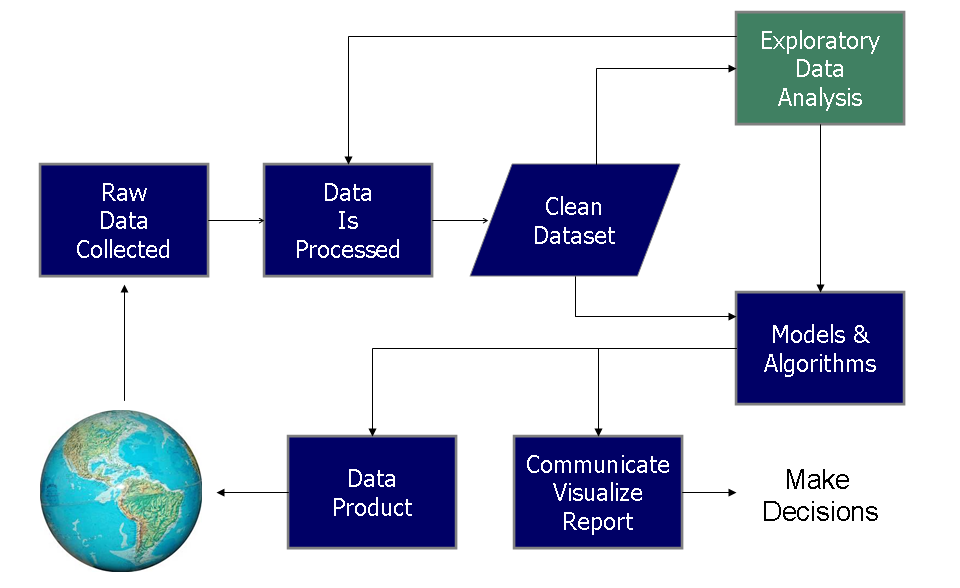
\includegraphics[width=\textwidth]{images/decisions}
\end{frame}


% EFFECTIVE COMMUNICATION
\begin{frame}
  \frametitle{Communicating effectively}
      \begin{itemize}  
        \item <1->\textcolor{hutton_green}{Understand the data}
        \begin{itemize}
          \item <2->size
          \item <2->cardinality
          \item <2->meaning
          \item <2->relationships
        \end{itemize}
        \item <1->\textcolor{hutton_blue}{Know (or be receptive to) the message}
        \begin{itemize}
          \item <3->what does pictorial representation mean?
          \item <3->match graphical relationships to data relationships
        \end{itemize}
        \item <1->\textcolor{hutton_purple}{Know your audience}
        \begin{itemize}
          \item <4->how do people process pictorial information
          \item <4->how does your audience process information
          \item <4->domain-specific representations
        \end{itemize}
      \end{itemize}  
\end{frame}
\subsection{Elementary perceptual tasks}
%% elementary_tasks.tex
%% Author: Leighton Pritchard
%% Copyright: James Hutton Institute
%% Elementary perceptual tasks, as in Cleveland & McGill (1984)

% ELEMENTARY PERCEPTUAL TASKS
\begin{frame}
  \frametitle{Elementary Perceptual Tasks
  \footnote{\tiny{\href{https://www.jstor.org/stable/2288400}{Cleveland \& McGill (1984) \textit{J. Am. Stat. Ass.}}}}
  }
  \textcolor{hutton_green}{The most basic visual tasks:}
  \begin{center}
    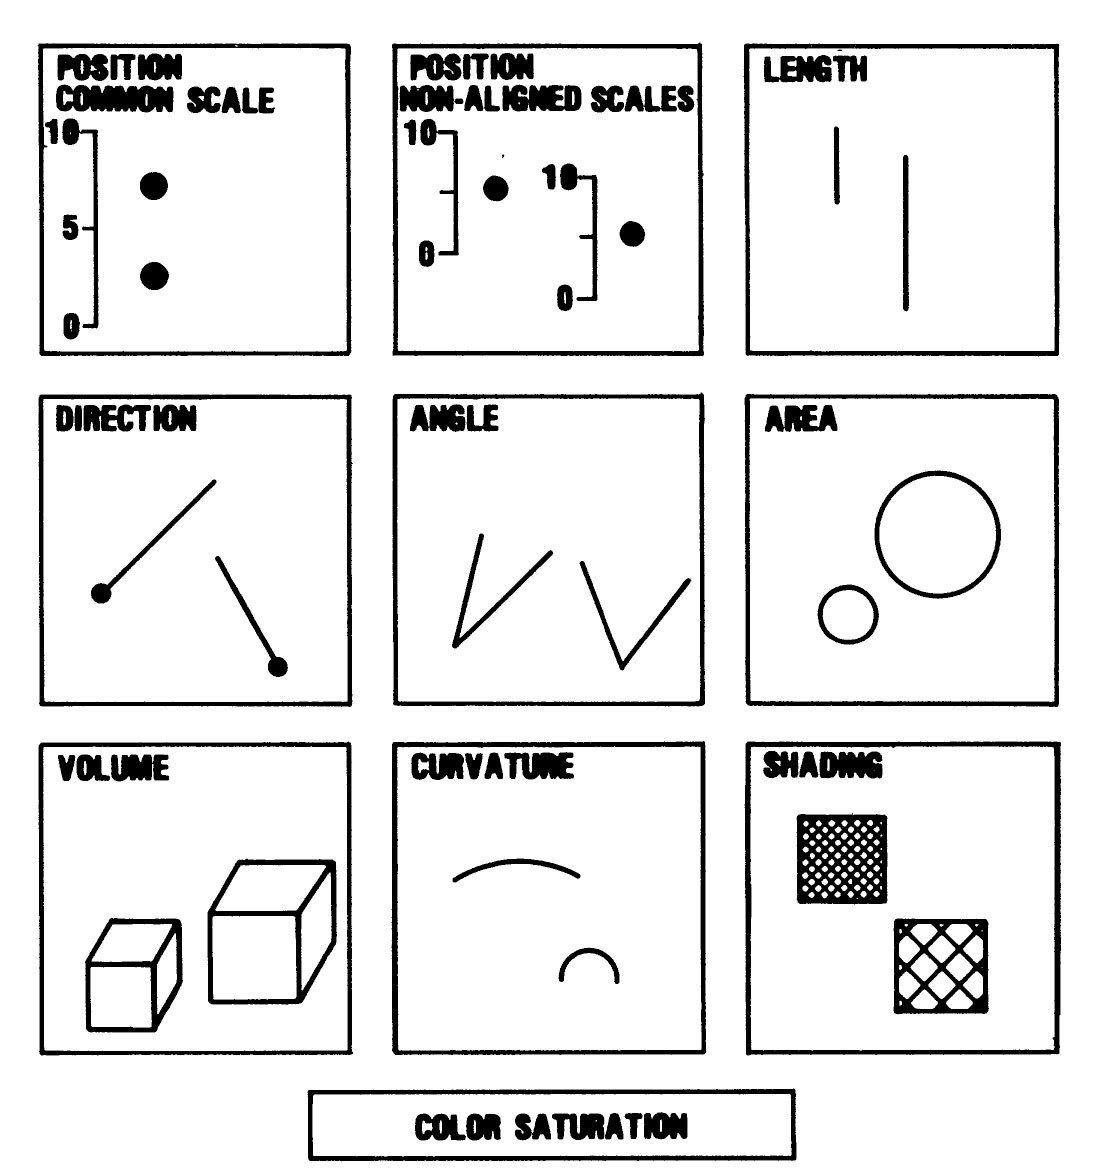
\includegraphics[height=0.7\textheight]{images/elementary_perceptual_tasks}
  \end{center}
\end{frame}

% WHAT IMPLEMENTS THESE?
\begin{frame}
  \frametitle{Implementations}
  \begin{columns}[T]
    \begin{column}{6cm}  
      \begin{alertblock}{Position: common scale}
        \begin{itemize}
          \item Scatterplot
          \item Bar Chart
        \end{itemize}
      \end{alertblock}
      \begin{block}{Angle}
        \begin{itemize}
          \item Pie Chart
          \item Do(ugh)nut Chart
        \end{itemize}  
      \end{block}
      \begin{alertblock}{Curvature}
        \begin{itemize}
          \item Arc Diagram
          \item Chord Diagram
        \end{itemize}
      \end{alertblock}
      \end{column}
    \begin{column}{4cm}  
      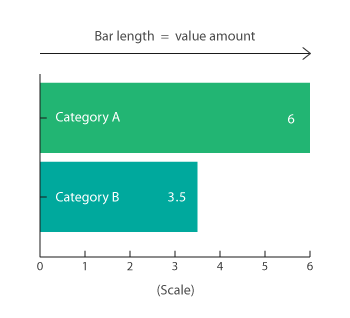
\includegraphics[width=0.65\textwidth]{images/bar_chart} \\
      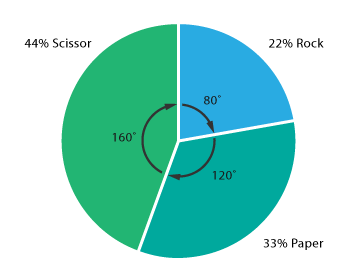
\includegraphics[width=0.65\textwidth]{images/pie_chart} \\
      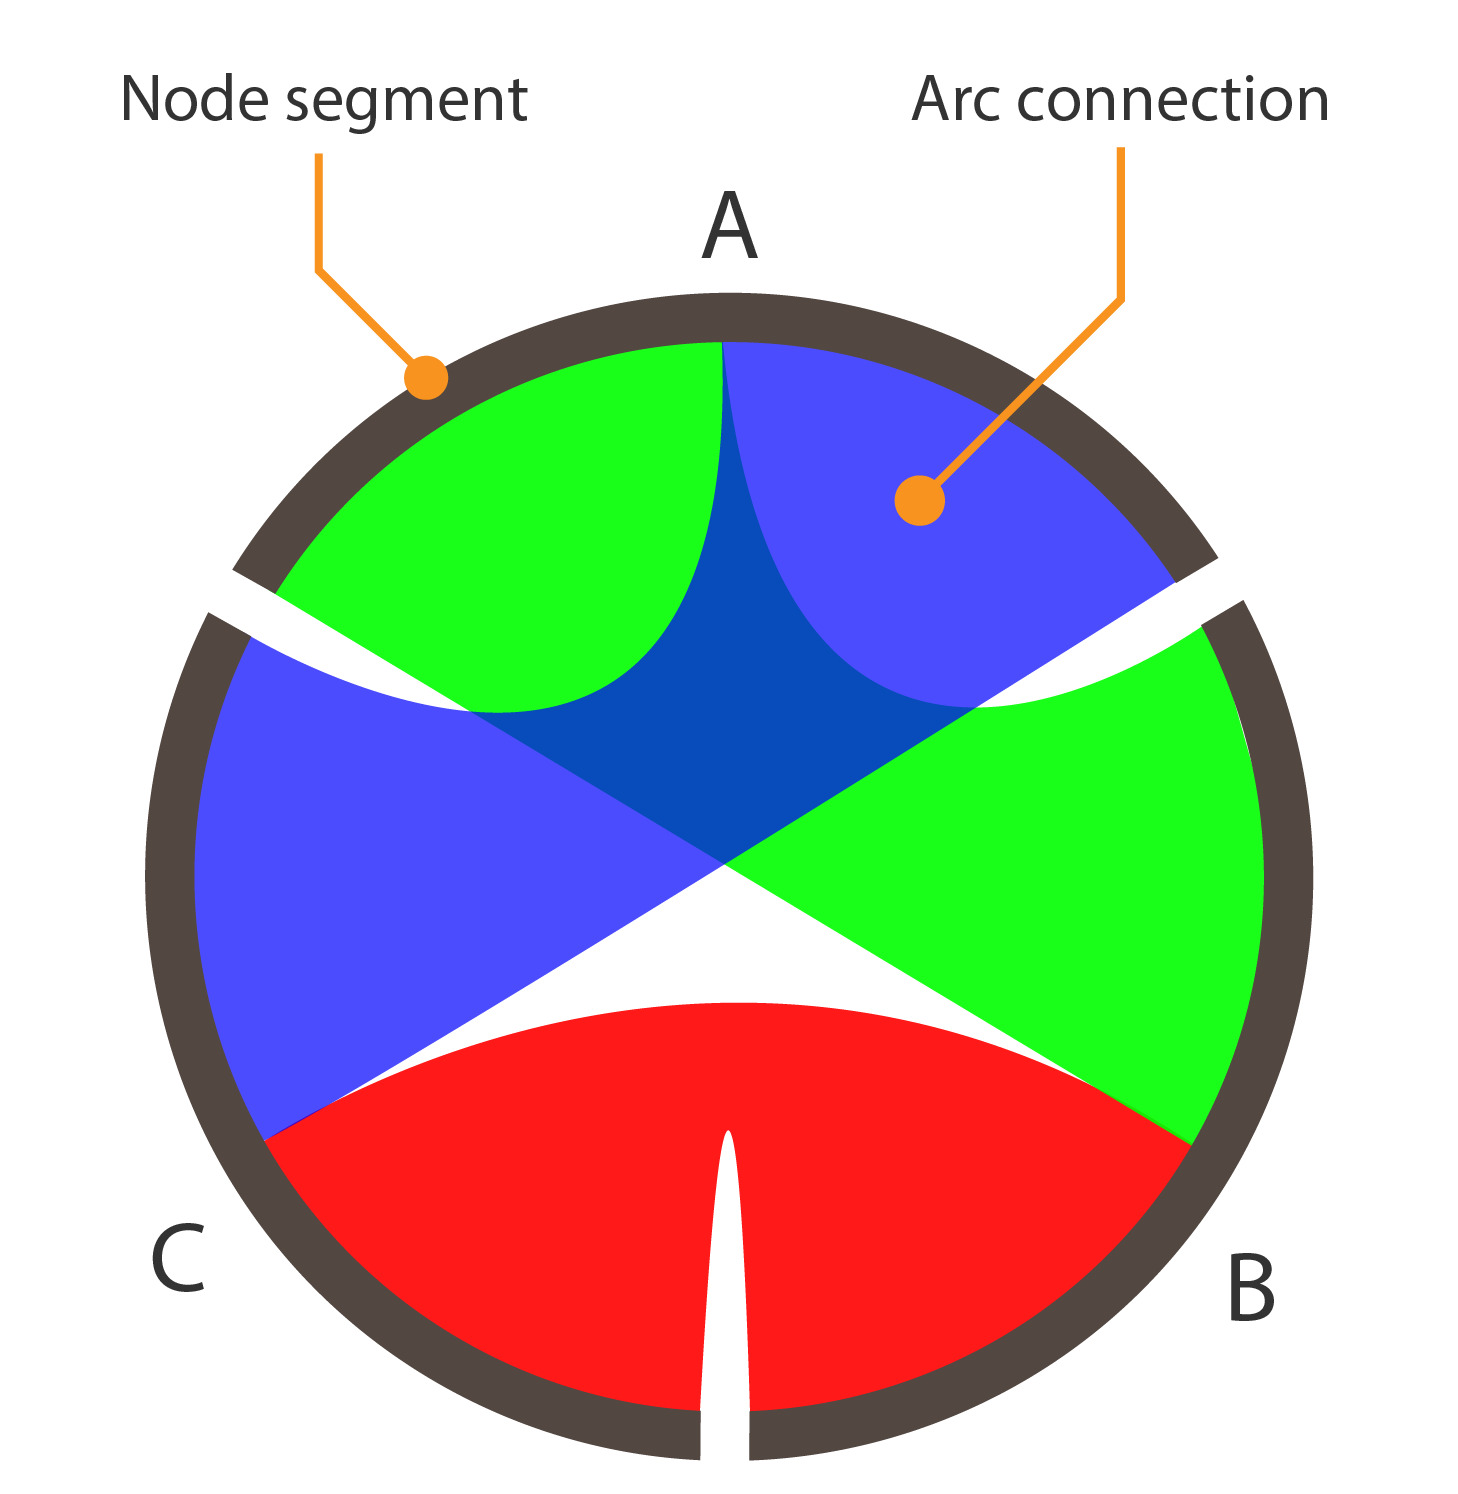
\includegraphics[width=0.65\textwidth]{images/chord_diagram}
    \end{column}
  \end{columns}      
\end{frame}



%%%
% SECTION: EVIDENCE-BASED REPRESENTATION
\section{Evidence-based representation}
\subsection{What representations work best?}
%% what_representation.tex
%% Author: Leighton Pritchard
%% Copyright: James Hutton Institute
%% Summary of Cleveland & McGill, Heer & Bostock studies

% WHAT WORKS BEST? EXPERIMENT
\begin{frame}
  \frametitle{What works best? Experiment
  \footnote{\tiny{\href{https://www.jstor.org/stable/2288400}{Cleveland \& McGill (1984) \textit{J. Am. Stat. Ass.}}}}  
  \footnote{\tiny{\href{http://vis.stanford.edu/files/2010-MTurk-CHI.pdf}{Heer \& Bostock (2010) \textit{CHI 2010}}}}
  }
    \textcolor{hutton_green}{Empirical measurements of interpretation}
    \begin{itemize}  
      \item Subjects shown graphs representing same data
      \item ($\log_2$) Error in subjects' accuracy compared by graph type
    \end{itemize}  
    \begin{alertblock}{Judgement types}
      \begin{itemize}
        \item 1-3: Position on a common scale (bar chart, stacked bar chart)
        \item 4-5: Length encoding (stacked bar chart)
        \item 6: Angle (pie chart)
        \item 7-9: Area (bubble chart, aligned rectangles, treemap) 
      \end{itemize}
    \end{alertblock}
\end{frame}

% WHAT WORKS BEST? RESULT
\begin{frame}
  \frametitle{What works best? Result
  \footnote{\tiny{\href{https://www.jstor.org/stable/2288400}{Cleveland \& McGill (1984) \textit{J. Am. Stat. Ass.}}}}  
  \footnote{\tiny{\href{http://vis.stanford.edu/files/2010-MTurk-CHI.pdf}{Heer \& Bostock (2010) \textit{CHI 2010}}}}
  }
  \begin{columns}[T]
    \begin{column}{5cm}
      \begin{itemize}
        \item \textcolor{hutton_green}{We have inherent biases that can distort information recovered}
        \item \textcolor{hutton_blue}{Position $>$ Angle $\approx$ Length $>$ Area}
        \item Accuracy plateaus as charts increase in size
        \item Gridlines improve accuracy
        \item \textcolor{hutton_purple}{Aspect ratios affect area judgements (squares worst)}
      \end{itemize}
    \end{column}
    \begin{column}{6cm}  
      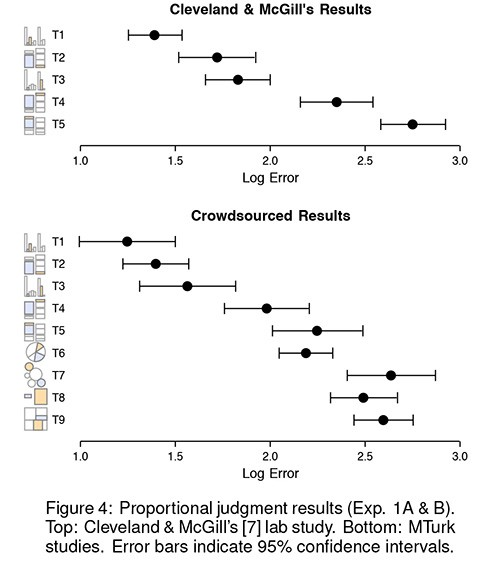
\includegraphics[width=1\textwidth]{images/proportional_results}    
    \end{column}
  \end{columns}      
\end{frame}
\subsection{Pie charts}
%% pie_charts.tex
%% Author: Leighton Pritchard
%% Copyright: James Hutton Institute
%% What does the evidence say about pie charts?

% PEOPLE HATE PIE CHARTS
\begin{frame}
  \frametitle{People hate pie charts}
    \begin{scriptsize}    
    \href{http://www.storytellingwithdata.com/blog/2011/07/death-to-pie-charts}{http://www.storytellingwithdata.com/blog/2011/07/death-to-pie-charts} \\
    \begin{alertblock}{especially Edward Tufte}
    A table is nearly always better than a dumb pie chart; the only worse design than a pie chart is several of them[...] pie charts should never be used. - \textit{"The Visual Display of Quantitative Information"}
    \end{alertblock}
    \end{scriptsize}
    \begin{center}
      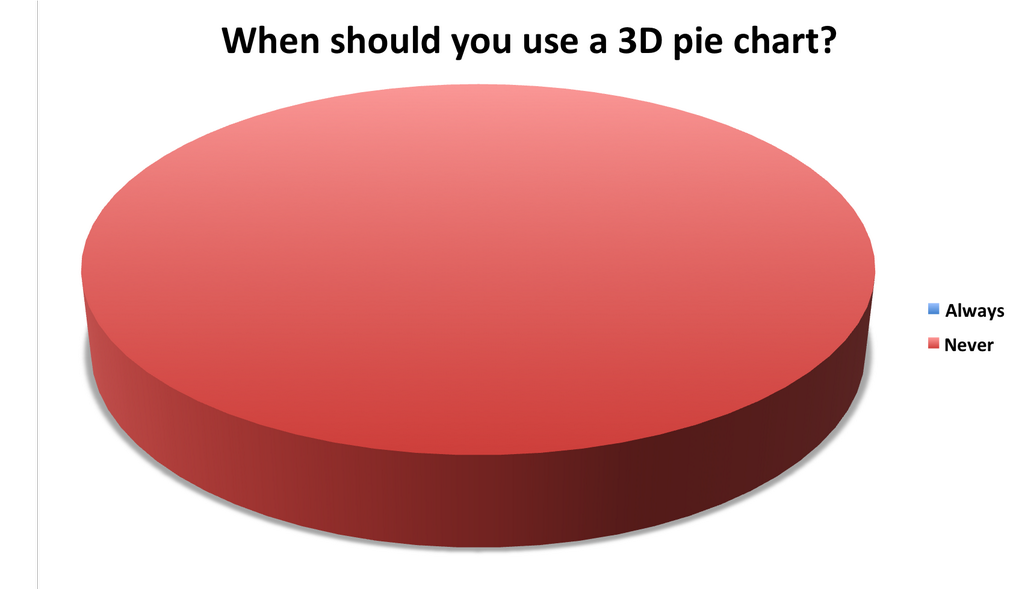
\includegraphics[height=0.5\textheight]{images/3d_pie_chart}
      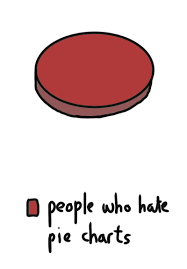
\includegraphics[height=0.5\textheight]{images/people_hate_pie_charts}
    \end{center}
\end{frame}

% BUT THEY HAVE USES
\begin{frame}
  \frametitle{"E pur si muove$\ldots$"
  \footnote{\tiny{\href{http://www.jstor.org/stable/2277140}{Eells (1926) \textit{J Am. Stat. Ass.}}}}
  \footnote{\tiny{\href{http://www.jstor.org/stable/2289447}{Simkin \& Hastie (1987) \textit{J Am. Stat. Ass.}}}}
  }
  \begin{scriptsize}
    \begin{alertblock}{For proportions of a whole:}
      \begin{itemize}
        \item Pie charts read as accurately as bar charts
        \item As number of components in the chart increases, bars are less efficient than pie charts
      \end{itemize}
    \end{alertblock}
  \end{scriptsize}
  \begin{center}
    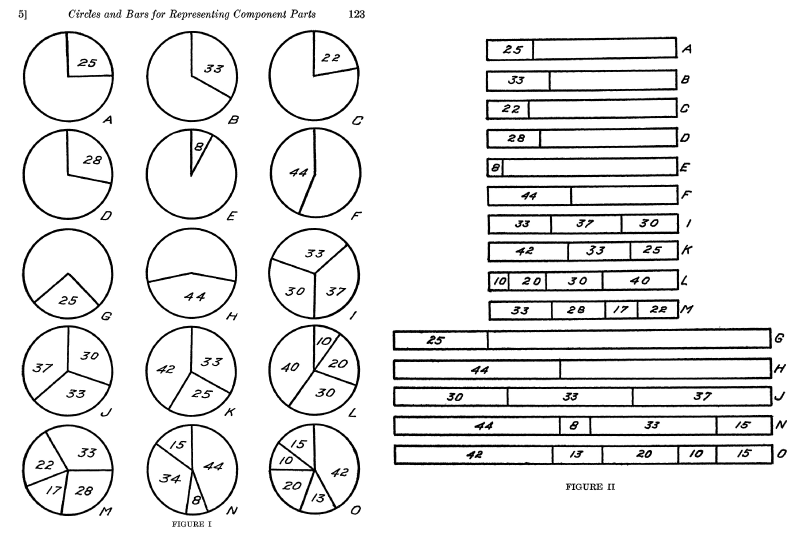
\includegraphics[height=0.45\textheight]{images/eells_experiment}    
  \end{center}
\end{frame}

\subsection{Bars and lines}
%% bar_charts.tex
%% Author: Leighton Pritchard
%% Copyright: James Hutton Institute
%% Do bar charts misrepresent data?

% DISDAIN FOR BAR CHARTS
\begin{frame}
  \frametitle{Bar charts are bad$\ldots$mmmkay?}
  \textcolor{hutton_green}{There is an ongoing backlash against bar charts} \\
  (and I'm not picking on Nick, he just tweets a lot$\ldots$)
  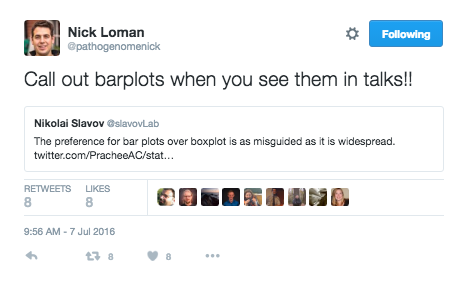
\includegraphics[height=0.3\textheight]{images/tweet_barchart}
  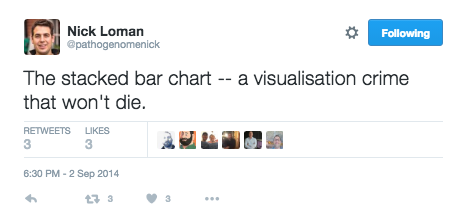
\includegraphics[height=0.3\textheight]{images/tweet_stackedbar} \\
  \textcolor{hutton_blue}{But are they really that bad?}
\end{frame}

% BAR/LINE INTERPRETATION 1
\begin{frame}
  \frametitle{Interpretation of bars and lines
  \footnote{\tiny{\href{http://link.springer.com/article/10.3758/BF03201236}{Zacks \& Tversky (1999) \textit{Mem. Cognit.}}}}
  }
  \begin{alertblock}{People interpret bars and lines differently}
  Experiment 1: In absence of context (arbitrary $X$, $Y$)
    \begin{itemize}
      \item \textbf{bars}: discrete comparison (24:0)
      \item \textbf{lines}: trend assessment (0:35)
    \end{itemize}
  \end{alertblock}
  \begin{center}
    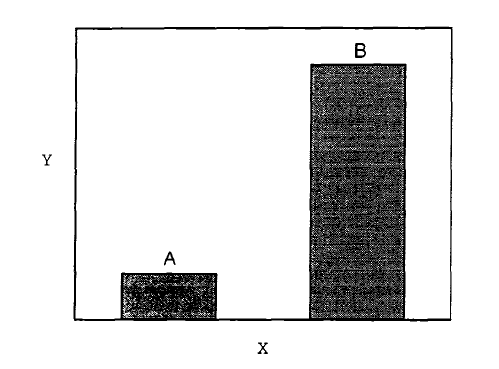
\includegraphics[width=0.4\textwidth,valign=t]{images/bars_v_lines_expt1a}    
    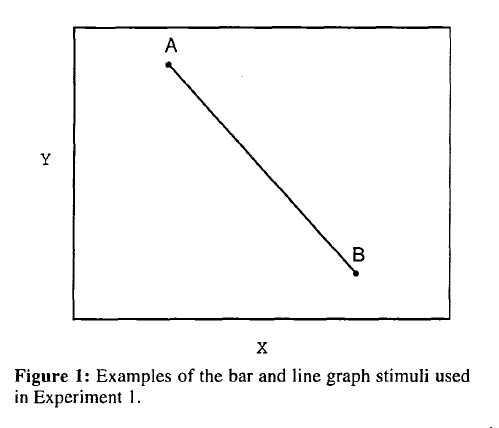
\includegraphics[width=0.4\textwidth,valign=t]{images/bars_v_lines_expt1b}  
  \end{center}
\end{frame}

% BAR/LINE INTERPRETATION 2
\begin{frame}
  \frametitle{Interpretation of bars and lines
  \footnote{\tiny{\href{http://link.springer.com/article/10.3758/BF03201236}{Zacks \& Tversky (1999) \textit{Mem. Cognit.}}}}
  }
  \begin{alertblock}{People interpret bars and lines differently}
  Experiment 2: With context (discrete or continuous data)\\
    \begin{center}
      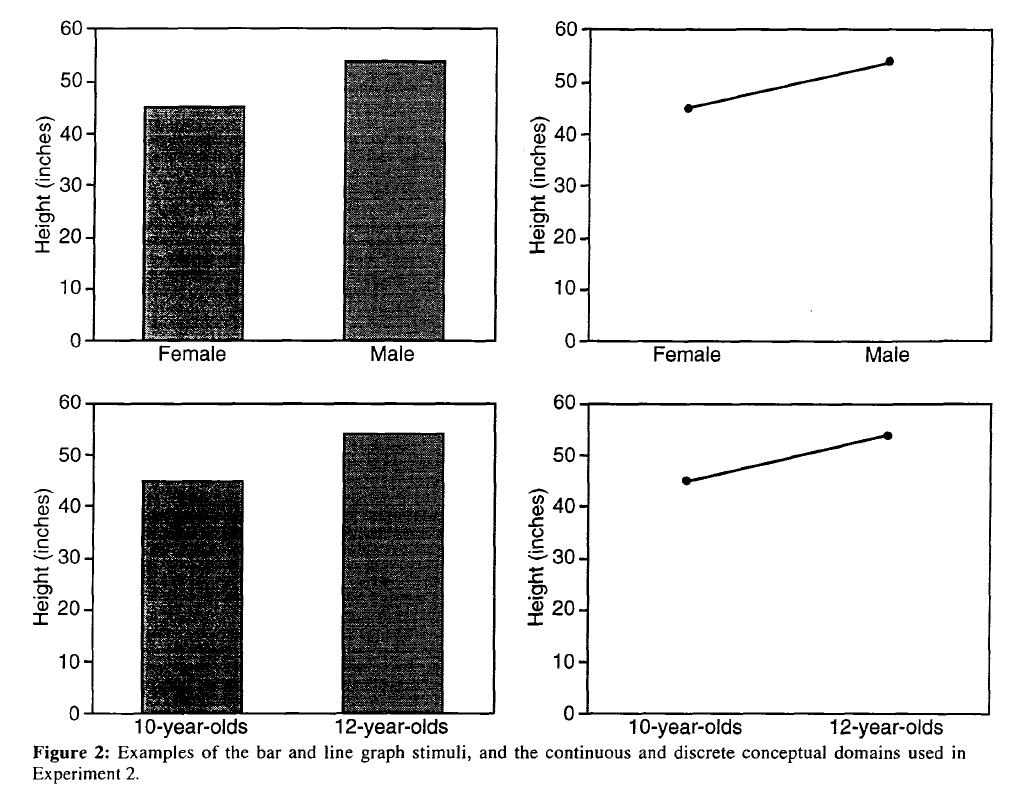
\includegraphics[height=0.4\textheight,valign=t]{images/bars_v_lines_expt2} \\
      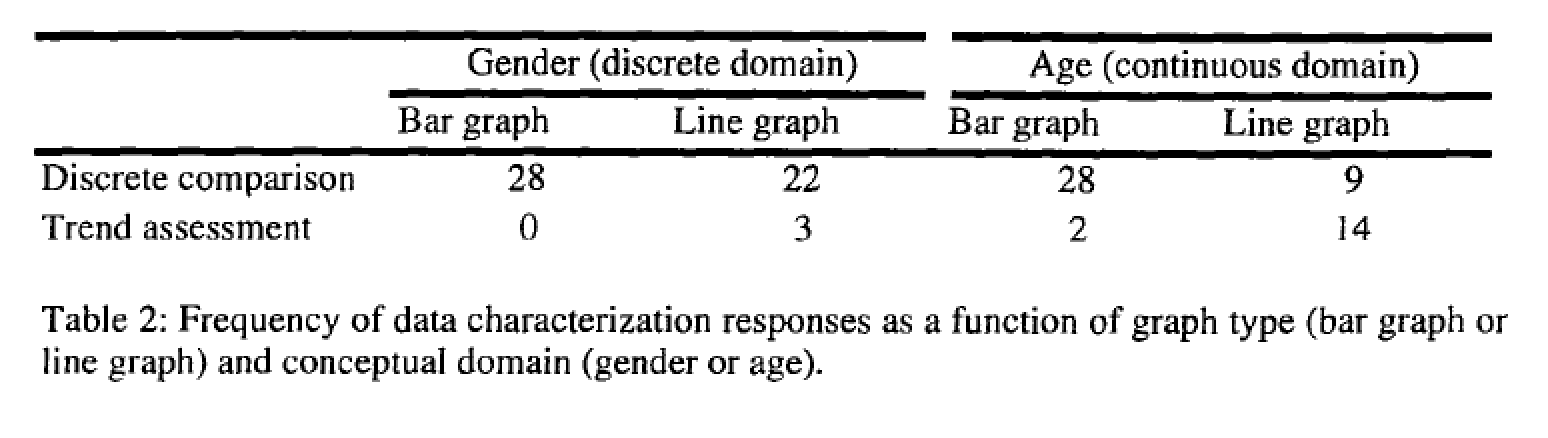
\includegraphics[width=0.7\textwidth,valign=t]{images/bars_v_lines_table}  
    \end{center}
  \end{alertblock}
  \begin{center}
  \end{center}
\end{frame}

% BAR/LINE CONCLUSIONS
\begin{frame}
  \frametitle{Bars \textit{ vs.} lines}
    \begin{itemize}  
      \item \textcolor{hutton_green}{People naturally interpret bar charts as categorical data}
      \item \textcolor{hutton_blue}{People naturally interpret line graphs as trends}
      \item \textcolor{hutton_purple}{Using bars for trend data or lines for categorical data can mislead the reader}
    \end{itemize}  
\end{frame}

% BAR CHARTS CAN MISLEAD
\begin{frame}
  \frametitle{Bar charts can mislead
  \footnote{\tiny{\href{http://dx.doi.org/10.1371/journal.pbio.1002128}{Weissgerber \textit{et al.} (2015) \textit{PLoS Biol.} doi:10.1371/journal.pbio.1002128}}}
  }
  \begin{columns}[T]
    \begin{column}{6cm}  
      \begin{itemize}  
        \item <1->\textcolor{hutton_green}{Do these bars differ in value?}
        \item <2->\textcolor{hutton_blue}{Bar charts represent data as a single point: lossy compression.}
        \item <2->\textcolor{hutton_purple}{Could different datasets give the same bar chart?}
      \end{itemize}  
    \end{column}
    \begin{column}{4cm}  
      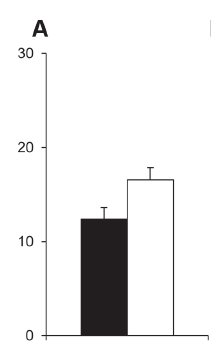
\includegraphics[width=1\textwidth]{images/weissgerber1}    
    \end{column}
  \end{columns}   
\end{frame}

% BARS ARE LOSSY COMPRESSION
\begin{frame}
  \frametitle{Bars are lossy compression
  \footnote{\tiny{\href{http://dx.doi.org/10.1371/journal.pbio.1002128}{Weissgerber \textit{et al.} (2015) \textit{PLoS Biol.} doi:10.1371/journal.pbio.1002128}}}
  }
    \begin{alertblock}{Bars hide detail:}
      \begin{itemize}
        \item Number of data points
        \item Variance of data points
        \item Distribution of data points (outliers, etc.)
      \end{itemize}
    \end{alertblock}
    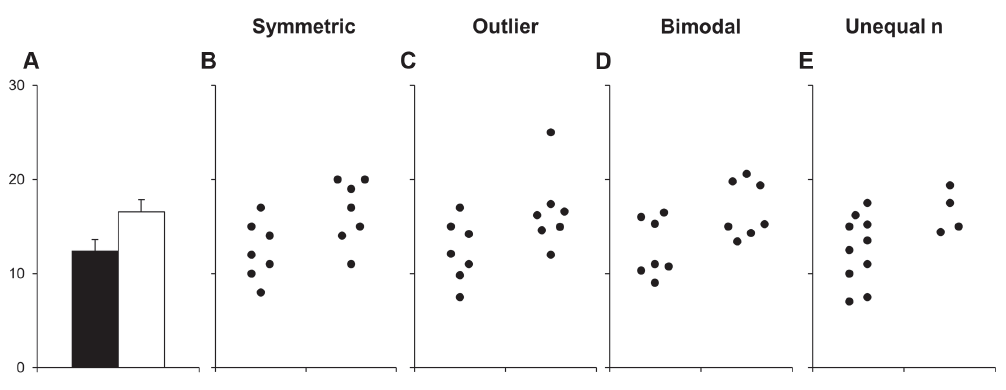
\includegraphics[width=1\textwidth]{images/weissgerber2}  
\end{frame}

% BARS MAY NOT GIVE GOOD STATISTICAL COMPARISONS
\begin{frame}
  \frametitle{Bars may mislead on statistics
  \footnote{\tiny{\href{http://dx.doi.org/10.1371/journal.pbio.1002128}{Weissgerber \textit{et al.} (2015) \textit{PLoS Biol.} doi:10.1371/journal.pbio.1002128}}}
  }
    \begin{alertblock}{Bars may imply incorrect test statistics:}
      Overlaps, outliers, covariates, sample sizes masked
    \end{alertblock}
    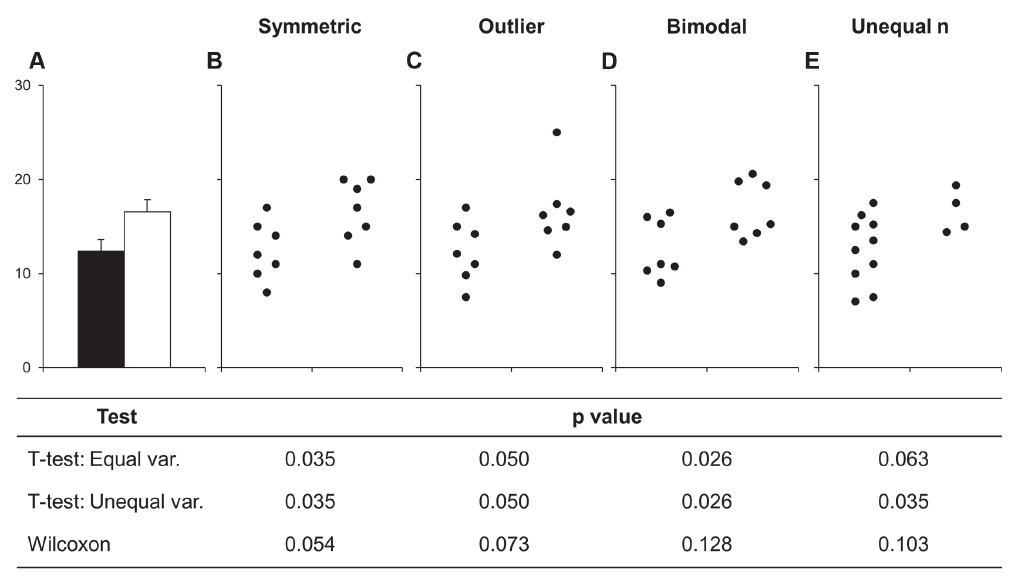
\includegraphics[width=1\textwidth]{images/weissgerber3}  
\end{frame}

% BARS DO NOT SHOW PAIRED DATA WELL
\begin{frame}
  \frametitle{Bars for paired data
  \footnote{\tiny{\href{http://dx.doi.org/10.1371/journal.pbio.1002128}{Weissgerber \textit{et al.} (2015) \textit{PLoS Biol.} doi:10.1371/journal.pbio.1002128}}}
  }
    \begin{alertblock}{Bars imply independence of data:}
    \end{alertblock}
    \begin{center}
      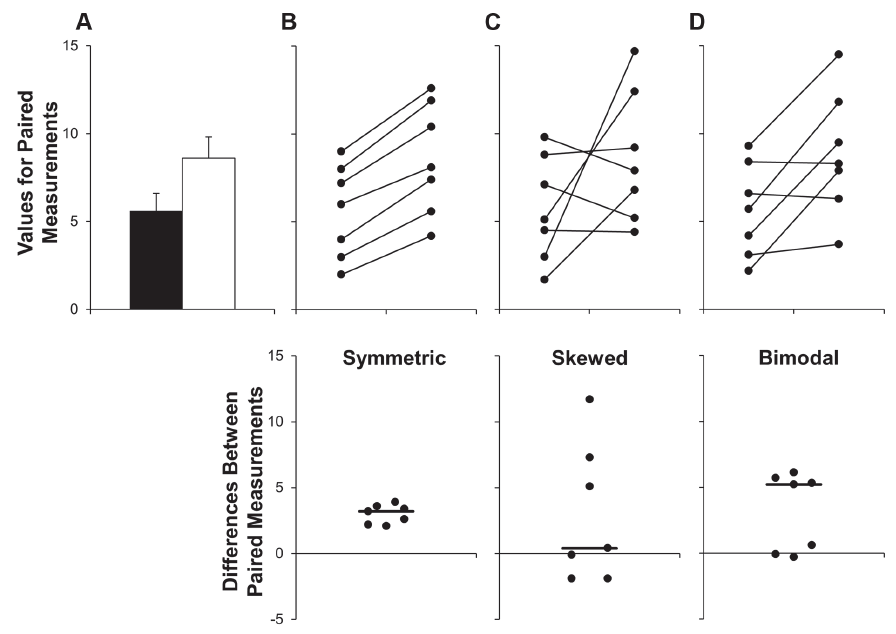
\includegraphics[width=0.8\textwidth]{images/weissgerber4}  
    \end{center}
\end{frame}

% BAR V SCATTER 1
\begin{frame}
  \frametitle{Better than bar charts?}
  \textcolor{hutton_green}{Bar chart with SE bars suggests group 2 is highest}
    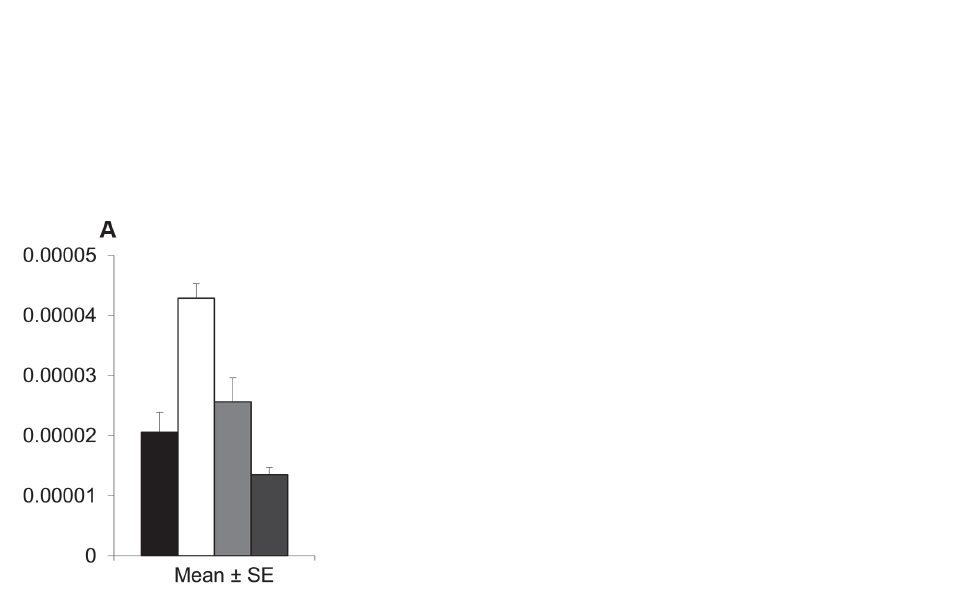
\includegraphics[width=1\textwidth]{images/weissgerber_bar_scatter1}    
\end{frame}

% BAR V SCATTER 2
\begin{frame}
  \frametitle{Better than bar charts?}
  \textcolor{hutton_blue}{Bar chart with SD bars suggests there is overlap}
    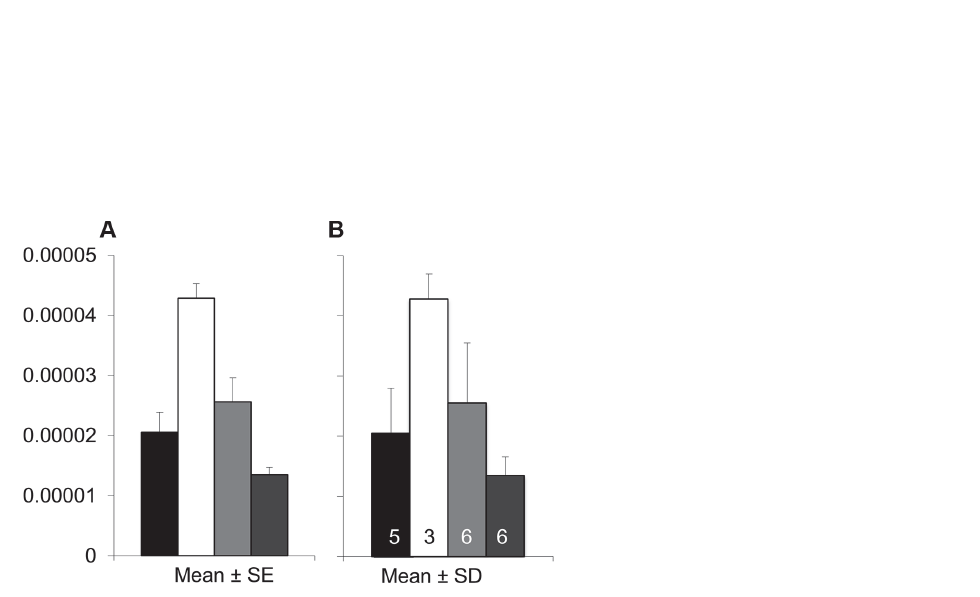
\includegraphics[width=1\textwidth]{images/weissgerber_bar_scatter2}    
\end{frame}

% BAR V SCATTER 3
\begin{frame}
  \frametitle{Better than bar charts?}
  \textcolor{hutton_purple}{Univariate scatterplots show sample sizes, outliers, variance}
    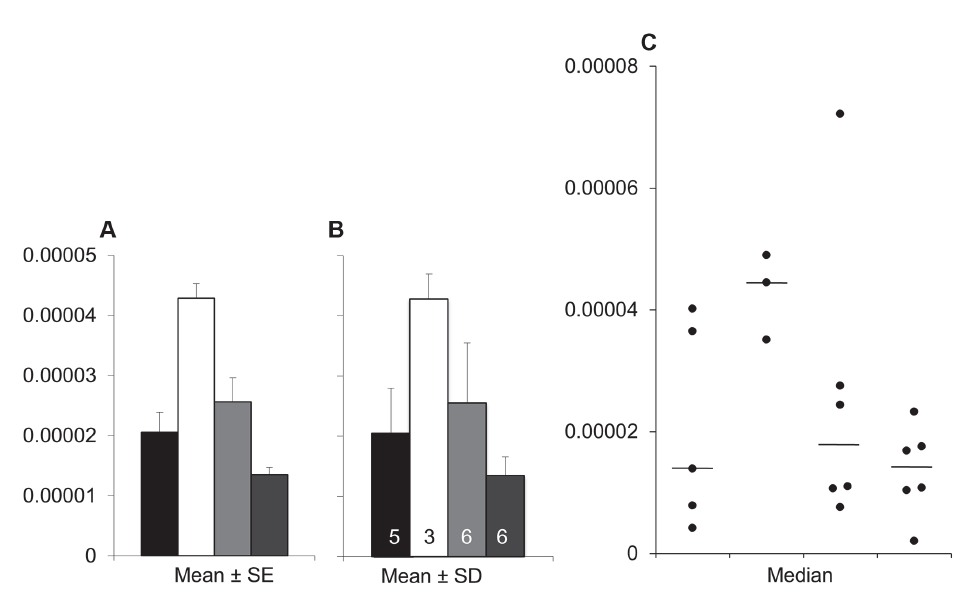
\includegraphics[width=1\textwidth]{images/weissgerber_bar_scatter3}    
\end{frame}
\subsection{Scatterplots}
%% scatterplots.tex
%% Author: Leighton Pritchard
%% Copyright: James Hutton Institute
%% Inferences of correlation from scatterplots are sensitive to presentation

% Frame template 
\begin{frame}
  \frametitle{Scatterplots
  \footnote{\tiny{\href{http://www.datavizcatalogue.com/}{http://www.datavizcatalogue.com/}}}
  }
  \begin{alertblock}{Scatterplots should be awesome:}
    \begin{itemize}
      \item Positions on common scale (lowest error representation)
      \item Show all data: outliers, sample sizes, trends, etc.
    \end{itemize}
  \end{alertblock}
  \begin{center}
    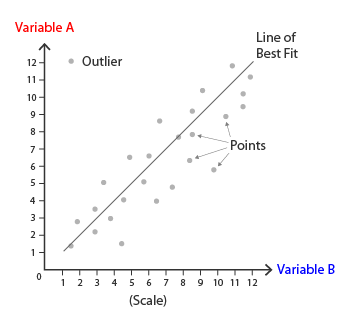
\includegraphics[width=0.5\textwidth,valign=t]{images/scatterplot1}
    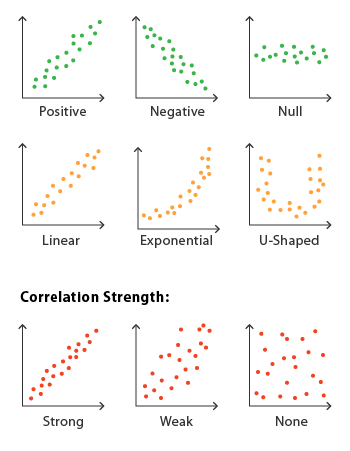
\includegraphics[width=0.33\textwidth,valign=t]{images/scatterplot2}
  \end{center}
\end{frame}

% Frame template 
\begin{frame}
  \frametitle{Framing affects interpretation
  \footnote{\tiny{\href{http://dx.doi.org/10.1126/science.216.4550.1138}{Cleveland \textit{et al.} (1982) \textit{Science} doi:10.1126/science.216.4550.1138}}}
  }
  \textcolor{hutton_green}{Point cloud size affects interpretation of correlation} \\
  \textcolor{hutton_blue}{(more diffuse interpreted as lower correlation coefficient)}
  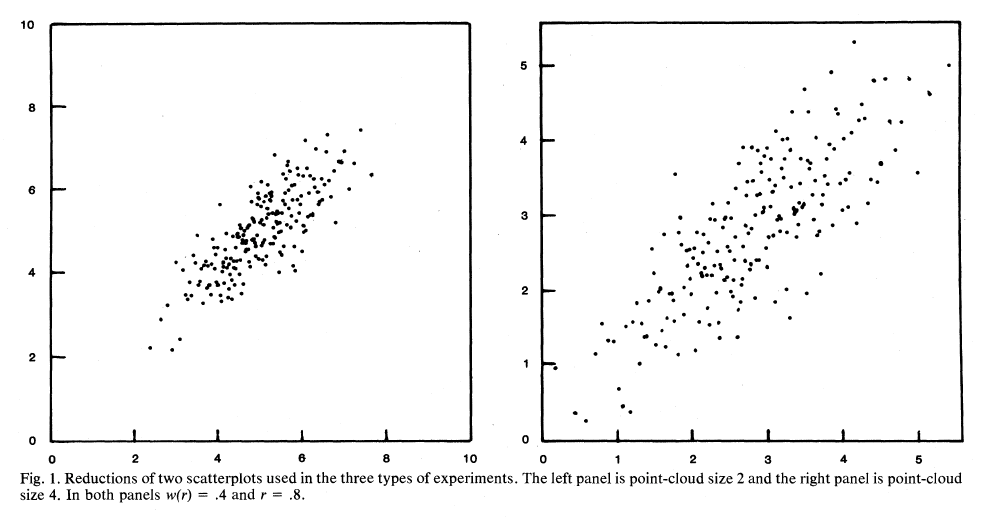
\includegraphics[width=1\textwidth]{images/scatterplot_framing}    
\end{frame}

% Frame template 
\begin{frame}
  \frametitle{Interpreting correlation is difficult
  \footnote{\tiny{\href{http://dx.doi.org/10.7717/peerj.589}{Fisher \textit{et al.} (2014) \textit{PeerJ} doi:10.7717/peerj.589}}}
  }
  \begin{alertblock}{People don't judge significance well}
    \begin{itemize}
      \item 47.4\% of significant relationships correctly classified
      \item 74.6\% of non-significant relationships correctly classified
    \end{itemize}
  \end{alertblock}
  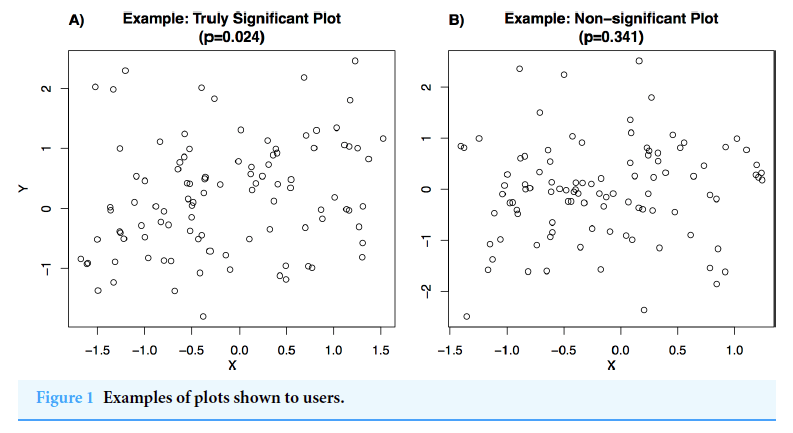
\includegraphics[width=0.5\textwidth]{images/scatterplot_fisher1}    
  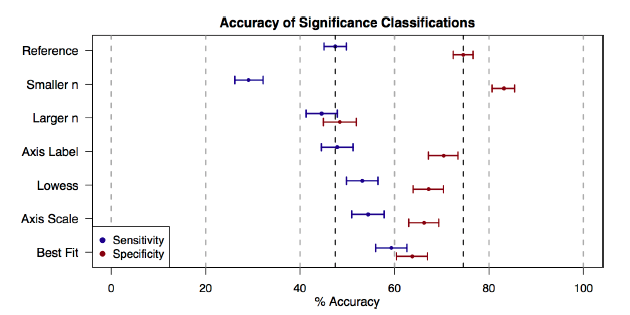
\includegraphics[width=0.5\textwidth]{images/scatterplot_fisher2}    
\end{frame}
\subsection{Interactive plots}
%% interactive_plots.tex
%% Author: Leighton Pritchard
%% Copyright: James Hutton Institute
%% The effect of latency on exploratory analysis

% LATENCY AFFECTS USAGE
\begin{frame}
  \frametitle{Latency affects usage}
  \begin{columns}[T]
    \begin{column}{5cm}  
    Increasing latency to 0.5s:
      \begin{itemize}  
        \item \textcolor{hutton_green}{decreases user activity}
        \item decreases dataset coverage
        \item \textcolor{hutton_blue}{reduces rate of hypothesis generation}
        \item \textcolor{hutton_purple}{changes data exploration strategy}
        \item reduces future interaction with other graphics
      \end{itemize}  
    \end{column}
    \begin{column}{5cm}  
      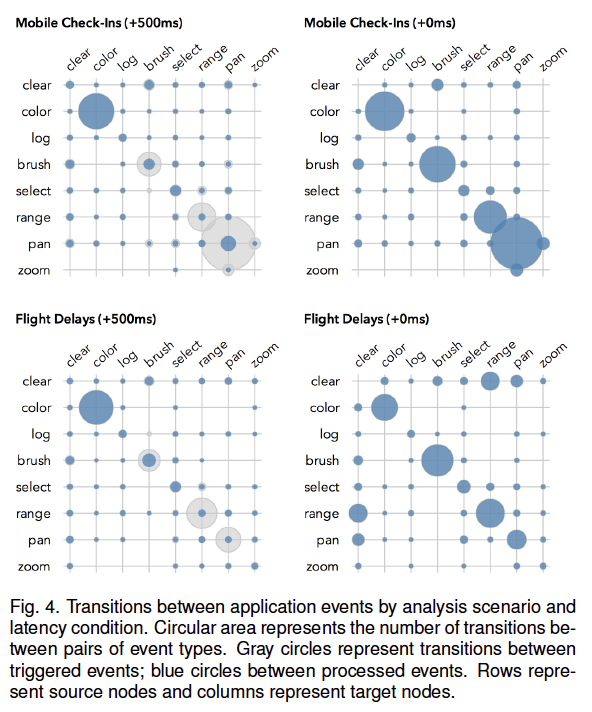
\includegraphics[width=1\textwidth]{images/latency}    
    \end{column}
  \end{columns}      
\end{frame}


%%%
% SECTION: BRIDGE TO PRACTICAL
\section{Hands-on session}
\subsection{Python libraries}
%%% python_libraries.tex
%% Author: Leighton Pritchard
%% Copyright: James Hutton Institute
%% The libraries used in these exercises

% PYTHON LIBRARIES
\begin{frame}
  \frametitle{Python libraries}
      \begin{itemize}  
        \item \textcolor{hutton_green}{Matplotlib} \href{http://matplotlib.org/}{http://matplotlib.org/} \\
         
\includegraphics[height=0.1\textheight]{images/matplotlib_logo}
        \item \textcolor{hutton_blue}{Seaborn} \href{https://stanford.edu/~mwaskom/software/seaborn/}{https://stanford.edu/~mwaskom/software/seaborn/} \\
          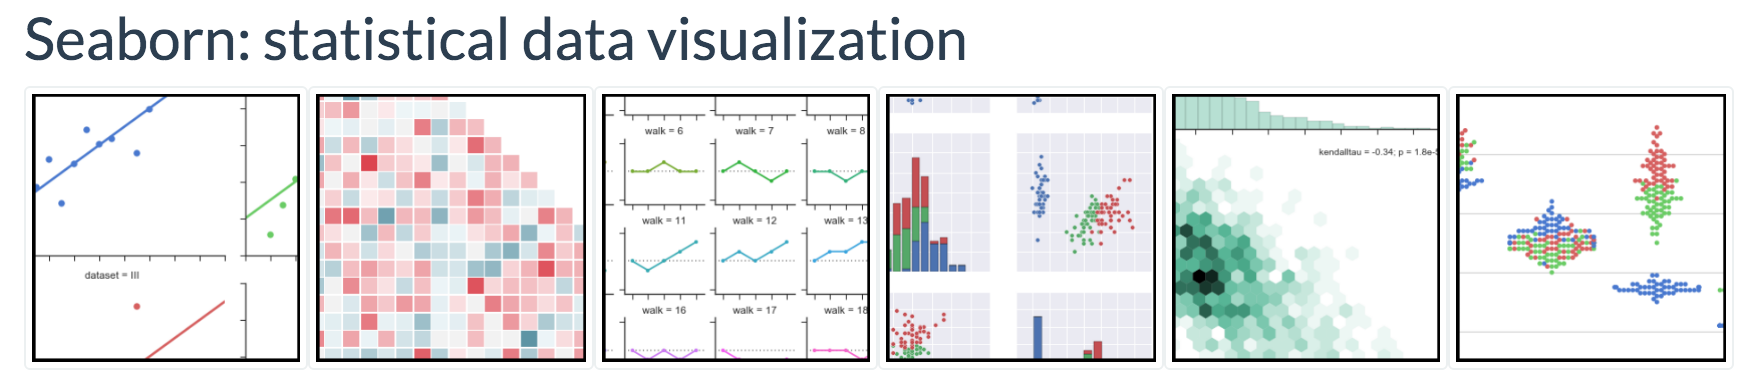
\includegraphics[height=0.1\textheight]{images/seaborn}
        \item \textcolor{hutton_purple}{ggplot} for Python \href{http://yhat.github.io/ggplot/}{http://yhat.github.io/ggplot/} \\
          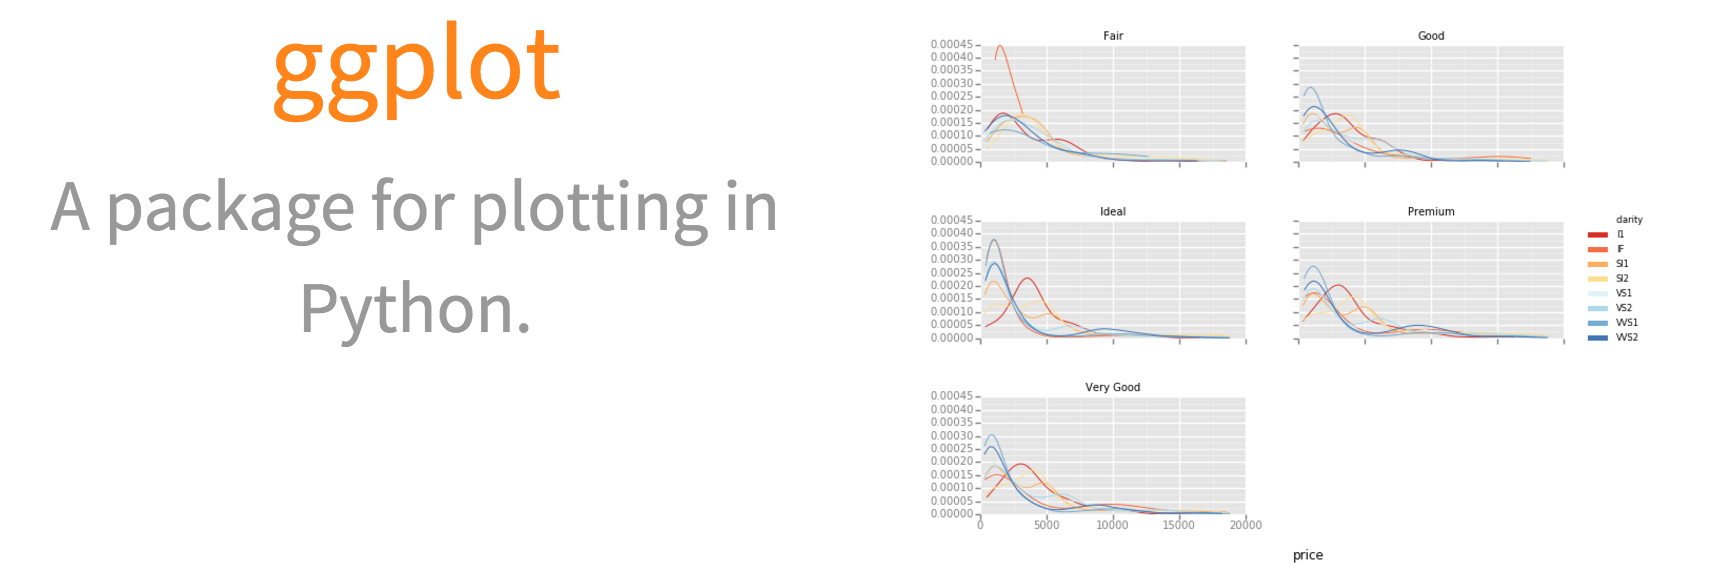
\includegraphics[height=0.1\textheight]{images/ggplot_python}
        \item \textcolor{red}{Bokeh} \href{http://bokeh.pydata.org/}{http://bokeh.pydata.org/} \\
          
\includegraphics[height=0.1\textheight]{images/bokeh_logo}
      \end{itemize}  
\end{frame}
\subsection{Exercises}
%% exercise_choices.tex
%% Author: Leighton Pritchard
%% Copyright: James Hutton Institute
%% Choice of exercises for the session

% EXERCISE CHOICES
\begin{frame}
  \frametitle{Exercise choices
  \footnote{\tiny{\href{https://github.com/widdowquinn/Teaching-Data-Visualisation}{https://github.com/widdowquinn/Teaching-Data-Visualisation}}}
  }
  \begin{scriptsize}
  \begin{columns}[T]
    \begin{column}{5.5cm}  
      \begin{itemize}  
        \item One-variable, continuous data\\
          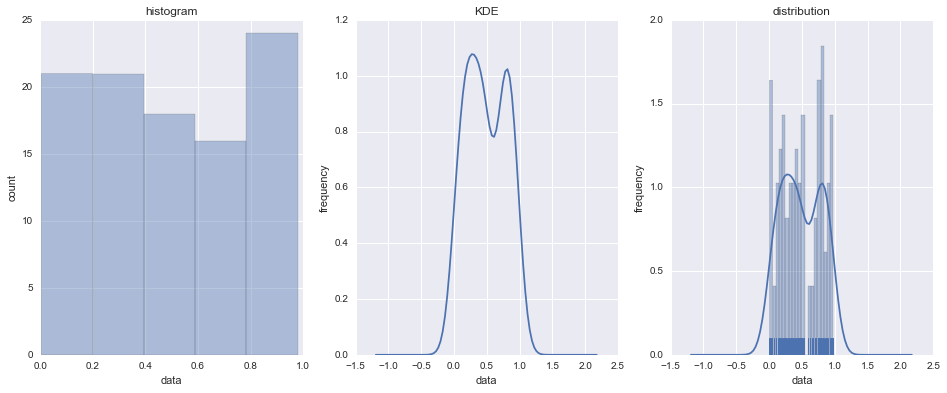
\includegraphics[height=0.15\textheight]{images/ex1}
        \item Grammar of Graphics\\
          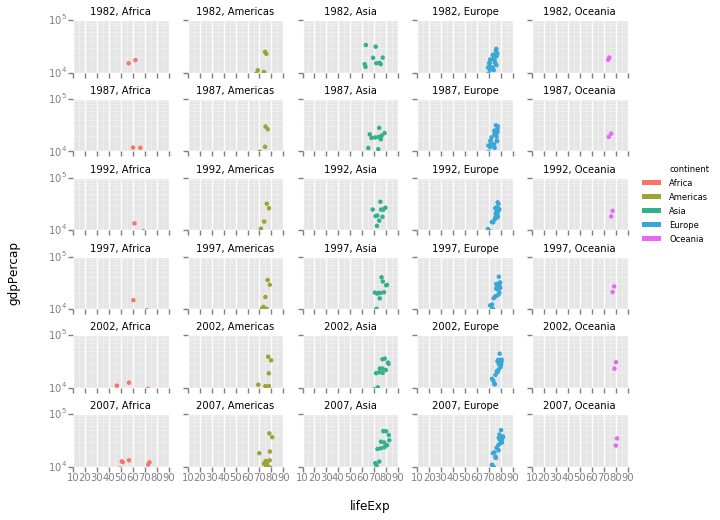
\includegraphics[height=0.15\textheight]{images/ex3}          
        \item Interactive map with bokeh\\
          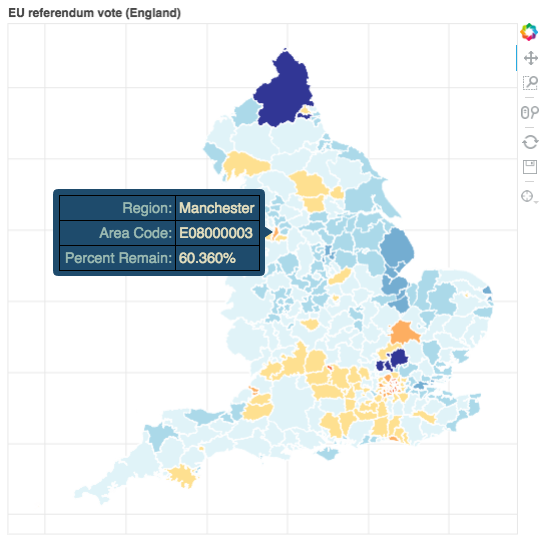
\includegraphics[height=0.15\textheight]{images/ex5}          
      \end{itemize}  
    \end{column}
    \begin{column}{5.5cm}  
      \begin{itemize}
        \item Two-variable, continuous x, y data\\
          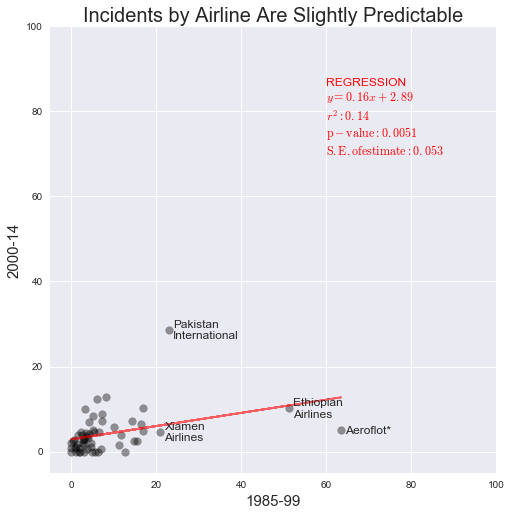
\includegraphics[height=0.15\textheight]{images/ex2}
        \item Arrays, colormaps, surface plots\\
          \includegraphics[height=0.15\textheight]{images/ex4}          
        \item Making movies\\
          \includegraphics[height=0.15\textheight]{images/ex6}
      \end{itemize}
    \end{column}
  \end{columns}   
  \end{scriptsize}   
\end{frame}

\subsection{Let's get started}
%% start_install.tex
%% Author: Leighton Pritchard
%% Copyright: James Hutton Institute
%% A slide to remind me to move on to the practical

% GETTING STARTED
\begin{frame}
  \frametitle{Let's get started
    \footnote{\tiny{\href{https://xkcd.com/1654/}{https://xkcd.com/1654/}}}
  }
  \begin{center}
    \includegraphics[height=0.7\textheight,valign=t]{images/universal_install_script}    
    \includegraphics[height=0.7\textheight,valign=t]{images/oreilly_stack_overflow}        
  \end{center}
\end{frame}


%%%
% SECTION: CONCLUSIONS
%\section{Conclusions}
%\subsection{General advice}
%%% general_advice.tex
%% Author: Leighton Pritchard
%% Copyright: James Hutton Institute
%% Collected wisdom

% CAVEAT
\begin{frame}
  \frametitle{A word of caution}
  \begin{alertblock}{Rules are there to be broken}
  There are good reasons for breaking nearly every rule of presentation at one time or another.
  \end{alertblock}
\end{frame}

% USE THE FULL AXIS
\begin{frame}
  \frametitle{Use the full axis}
  \textcolor{hutton_blue}{but does difference from initial value matter more than absolute value?}
  \begin{center}
    \includegraphics[width=0.35\textwidth,valign=c]{images/truncated_y}
    \includegraphics[width=0.65\textwidth,valign=c]{images/non-connected-axes}    
  \end{center}
\end{frame}

% SIMPLIFY
\begin{frame}
  \frametitle{Simplify to your message}
  \begin{center}
    \includegraphics[width=0.45\textwidth,valign=t]{images/datavis_overcomplex}
    \includegraphics[width=0.55\textwidth,valign=t]{images/simplify}    
  \end{center}
\end{frame}

%%%
% SECTION: Acknowledgements
%\section{Acknowledgements}
%\input{sections/acknowledgements}

%%%
% LICENCE FOR REUSE
%% licence.tex
%% Author: Leighton Pritchard
%% Copyright: James Hutton Institute
%% These slides describe the licence for reuse of these slides and
%% materials

%
\begin{frame}
  \frametitle{Licence: CC-BY-SA}
  By: Leighton Pritchard \\[0.5cm]
  This presentation is licensed under the Creative Commons Attribution ShareAlike license \\
  \href{https://creativecommons.org/licenses/by-sa/4.0/}{https://creativecommons.org/licenses/by-sa/4.0/}
\end{frame}

% etc
\end{document}